\setchapterpreamble[u]{\margintoc}
\glsresetall % reset glossary

\chapter{Design of real-size aeronautical wing structures} \label{chap:07}

Ultralight trusses offer a compelling solution for the development of innovative aerostructures due to their exceptional aeroelastic properties and high stiffness-to-weight ratio. These structures align well with the optimization formulations discussed in previous chapters. Opgenoord \sidecite{opgenoord_aeroelastic_2018, opgenoord_design_2019} proposed a two-step sequential optimization approach to reduce the weight of truss wings. Initially, they generated a ground structure with varying nodal densities based on the stress field, followed by a sizing optimization algorithm to determine the cross-sectional areas, considering stress, local buckling, and aeroelastic constraints. Shahabsafa \sidecite{shahabsafa_novel_2018}, on the other hand, took a different approach, employing discrete cross-sectional areas and a \gls{milo} sizing optimization algorithm to address the complexities of the problem. However, by solely focusing on modifying the component sizes, the opportunity to optimize the overall truss topology is missed, limiting the potential\marginnote{Part of the content presented in this chapter has been published as:\\Stragiotti, E. et al. (2024) "Efficient 3D truss topology optimization for aeronautical structures", in \textit{Structural and Multidisciplinary Optimization}~\cite{stragiotti_efficient_2024}.} for further weight savings. Moreover, none of these studies evaluated the fabricability of the proposed designs, highlighting the potential benefits of modularity in addressing these aspects.

In the preceding chapters, our focus was on the development of optimization methods for both monolithic and modular structures, which were then applied to two- and three-dimensional academic load cases. In this chapter, we aim to validate the proposed optimization algorithms by applying them to real-world engineering problems in the aeronautical domain. Firstly, to evaluate computational efficiency and validate the strategy outlined in \chpref{chap:04}, we optimize a monolithic three-dimensional wingbox test case based on the \gls{crm}, considering multiple load cases and two discretization refinements. Subsequently, we apply the modular algorithm introduced in \chpref{chap:06} to a UAV-sized wing utilizing an extruded NACA 0012 profile.

The optimization cases presented in this section are performed on a notebook equipped with an Intel\textsuperscript{\textregistered} Core™ i5-9400H Processor @ \qty{2.50}{GHz} (4 cores) and \qty{16}{GB} of RAM. 

\section{3D CRM wingbox with multiple load cases}
In this section, the monolithic optimization strategy presented in \chpref{chap:04} is used to optimize a real-sized wingbox, to validate its ability to work on large, three-dimensional structures with more candidate members compared to the precedent test cases. The structure is based on the jig (undeformed) shape of the wingbox of the NASA \gls{crm} \sidecite{brooks_benchmark_2018}. The structure is submitted to three different load cases: +2.5 g maneuver (LC\_1), -1 g maneuver (LC\_2), and cruise with gust +1.3 g (LC\_3). The nodes of the bounding volume and the loads used are provided by Fakhimi \etal \sidecite{fakhimi_discrete_2021}, where a detailed discussion on how they are evaluated can be found. The ground structure of the test case is presented in \figref{fig:07_crm315_x0}. Additionally, the load cases and the starting point, of all the presented test cases are available in the reference data set \sidecite{enrico_stragiotti_truss_2023}.

The optimization utilizes an aluminum alloy, with mechanical properties detailed in \tabref{tab:07_CRM_mat}. To ensure a conservative design, we incorporated safety factors (\textit{sf}) associated with each load case. These safety factors are integrated into the formulation by reducing the maximum stress and buckling allowables by factors of 1.5, 1.5, and 2.67\sidenote{They are the same values used by Fakhimi \etal \cite{fakhimi_discrete_2021}} for the three considered load cases, respectively. The cross-sections are assumed circular with the cross-sectional buckling parameter $s = \pi E/4$. The optimization is carried only on the wingbox, the internal structure of the wing, and there is no influence of the skin on the optimization.
\begin{margintable}
    \small
    \centering
    \begin{tabular}{cc}
    \toprule
    \textbf{Parameter}        & \textbf{Value} \\ \midrule
    $E$              & \qty{69}{GPa}     \\
    $\sigma_\text{c}, \sigma_\text{t}$ & $\pm $\qty{270}{MPa} \\
    $\rho$              & \qty{2.7}{\gram\per\cubic\centi\metre}   \\
    \bottomrule
    \end{tabular}
    \caption{Material data used for the CRM optimization.}
    \label{tab:07_CRM_mat}
\end{margintable}

The optimization runs are performed using the Python package CVXPY 1.2.2 \sidecite{diamond_cvxpy_2016} with the ECOS 2.0.7 \sidecite{domahidi_ecos_2013} solver to solve the relaxed \gls{lp} Problem \eqref{eq:04_optim_no_constr_lp}. The \gls{nlp} Problem \eqref{eq:04_optim_complete} is solved using cyipopt \sidecite{Moore_Mechmotum}, a Python wrapper for IPOPT 3.14.11 \sidecite{wachter_implementation_2006}, a large-scale nonlinear optimization package using PARDISO 6.0 \sidecite{alappat_recursive_2020} as the linear solver. The stopping criterion used for the \gls{slp} and \gls{nlp} optimisations are $\norm{\Delta \vect{x}}_\infty \leq \text{tol}_{slp}  \text{, and } \norm{\Delta_{\text{NLP}}}_\infty \leq \text{tol}_{nlp}$, with $\text{tol}_{slp}=10^{-6}$ and $\text{tol}_{nlp}=10^{-4}$ respectively. $\Delta_{\text{NLP}}$ represents the scaled \gls{nlp} error, a more comprehensive value used by IPOPT to take into account the optimality of the solution and the constraints violation. The reinitialization magnitude parameter $\vect{\phi}$ is set up using \eqref{eq:04_phi} \marginnote{\eqref{eq:04_phi} reads: $$\phi_n = \phi_{n-1}^\beta \quad \forall n \in [1,\dots,n_{\text{max}}],$$ with $\phi_0=0.8$ and $\beta=2$.}, leading to $\vect{\phi} = \left[ 0.8000, 0.6400, 0.4096, 0.1677, 0.0281 \right]$ for the five reinitialization calls of 2S-5R. The full list of parameters used to set up the variable scaling, the SLP optimization, the reinitialization, and the NLP optimization is listed in \tabref{tab:04_param}.

\subsection{Advanced thresholding}
As the \gls{crm} is a large and thin structure that presents a noticeable difference in load magnitude between the tip and the root of the wingbox, the quantities of interest of the optimization span different orders of magnitude (from \unit{m^2} to \unit{mm^2}, and\marginnote{\eqref{eq:04_thr} reads: $$a_i<a_{\text{thr}} \; \forall i, \text{ with }a_{\text{thr}} = \chi \; \max(\tilde{\vect{a}}^*)$$} from \unit{MN} to \unit{N}). For that reason, the choice of the cross-sectional area threshold value $\chi$ defined in \eqref{eq:04_thr} and used to simplify the initial \gls{nlp} ground structure using the SLP solution $\tilde{\vect{a}}^*$ is crucial. Taking a high value (such as $\chi = 10^{-4}$, restraining the cross-sectional areas of the solution from \unit{m^2} to \unit{cm^2}) would mean possibly canceling out bars fundamental for the nodal force equilibrium in the less loaded parts of the wing (wing tip and the central part of the wing's section near the root). By contrast, a low value (such as $\chi=10^{-9}$) would permit the correct simulation of the mechanical response of the structure, but it would lead to a very high number of candidate bars and, thus, longer computational time and harder convergence for the \gls{nlp} phase. For that reason, $\chi$ is set to an intermediate value ($\chi=10^{-6}$), eliminating all the bars under the value $a_{\text{thr}}$, but an additional check is performed before proceeding to the thresholding. The bars under the threshold $a_{\text{thr}}$ are sorted in ascending order of cross-sectional area and, starting from the smallest one, we iteratively check via a \gls{fea} that the difference between the force and displacement fields before and after the bar removal remains below a certain bound. In the present study we used the following: $\norm{\Delta q}_{\infty}<\qty{10}{N}$ and $\norm{\Delta U}_{\infty}<\qty{1}{cm}$.
\subsection{Numerical optimization of the CRM wingbox}    
    \begin{figure*}
        \centering
        \subcaptionbox{\label{fig:07_crm315_x0}}{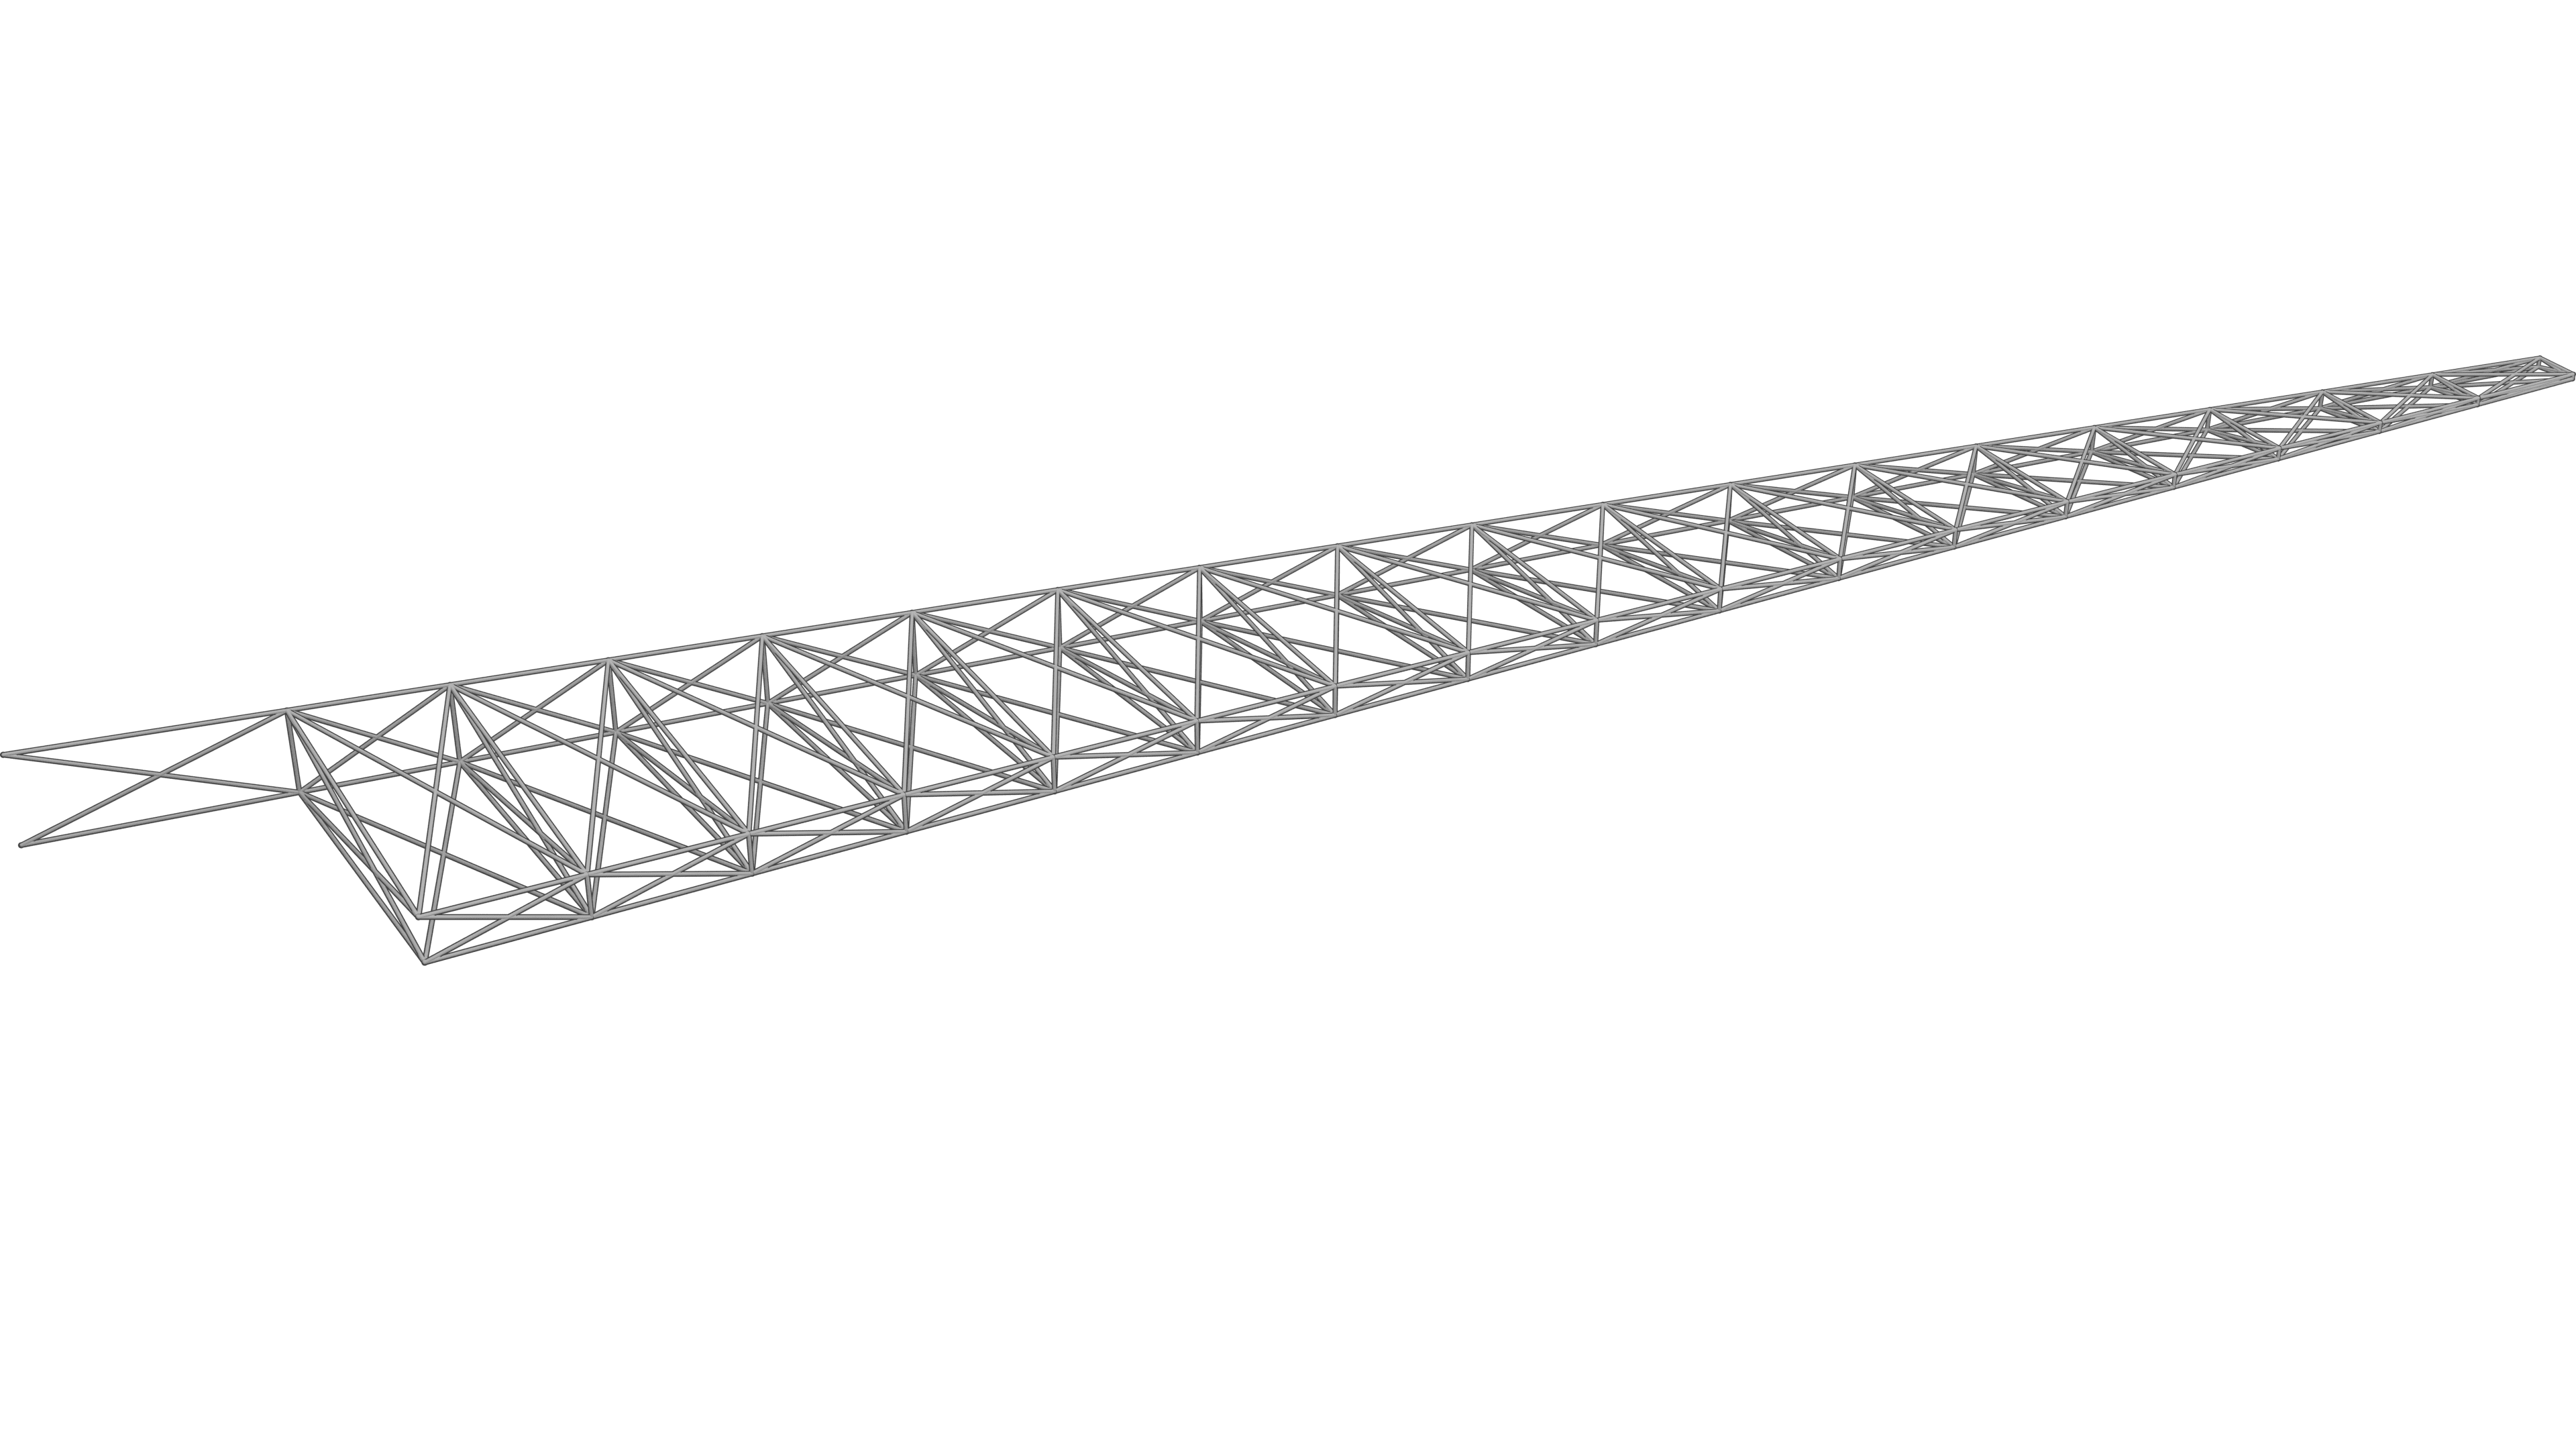
\includegraphics[width=0.45\linewidth]{figures/07_aeronautic/14a_00_Topology_x0_iso.png}}
        \bigskip
        \subcaptionbox{\label{fig:07_crm2317_x0}}{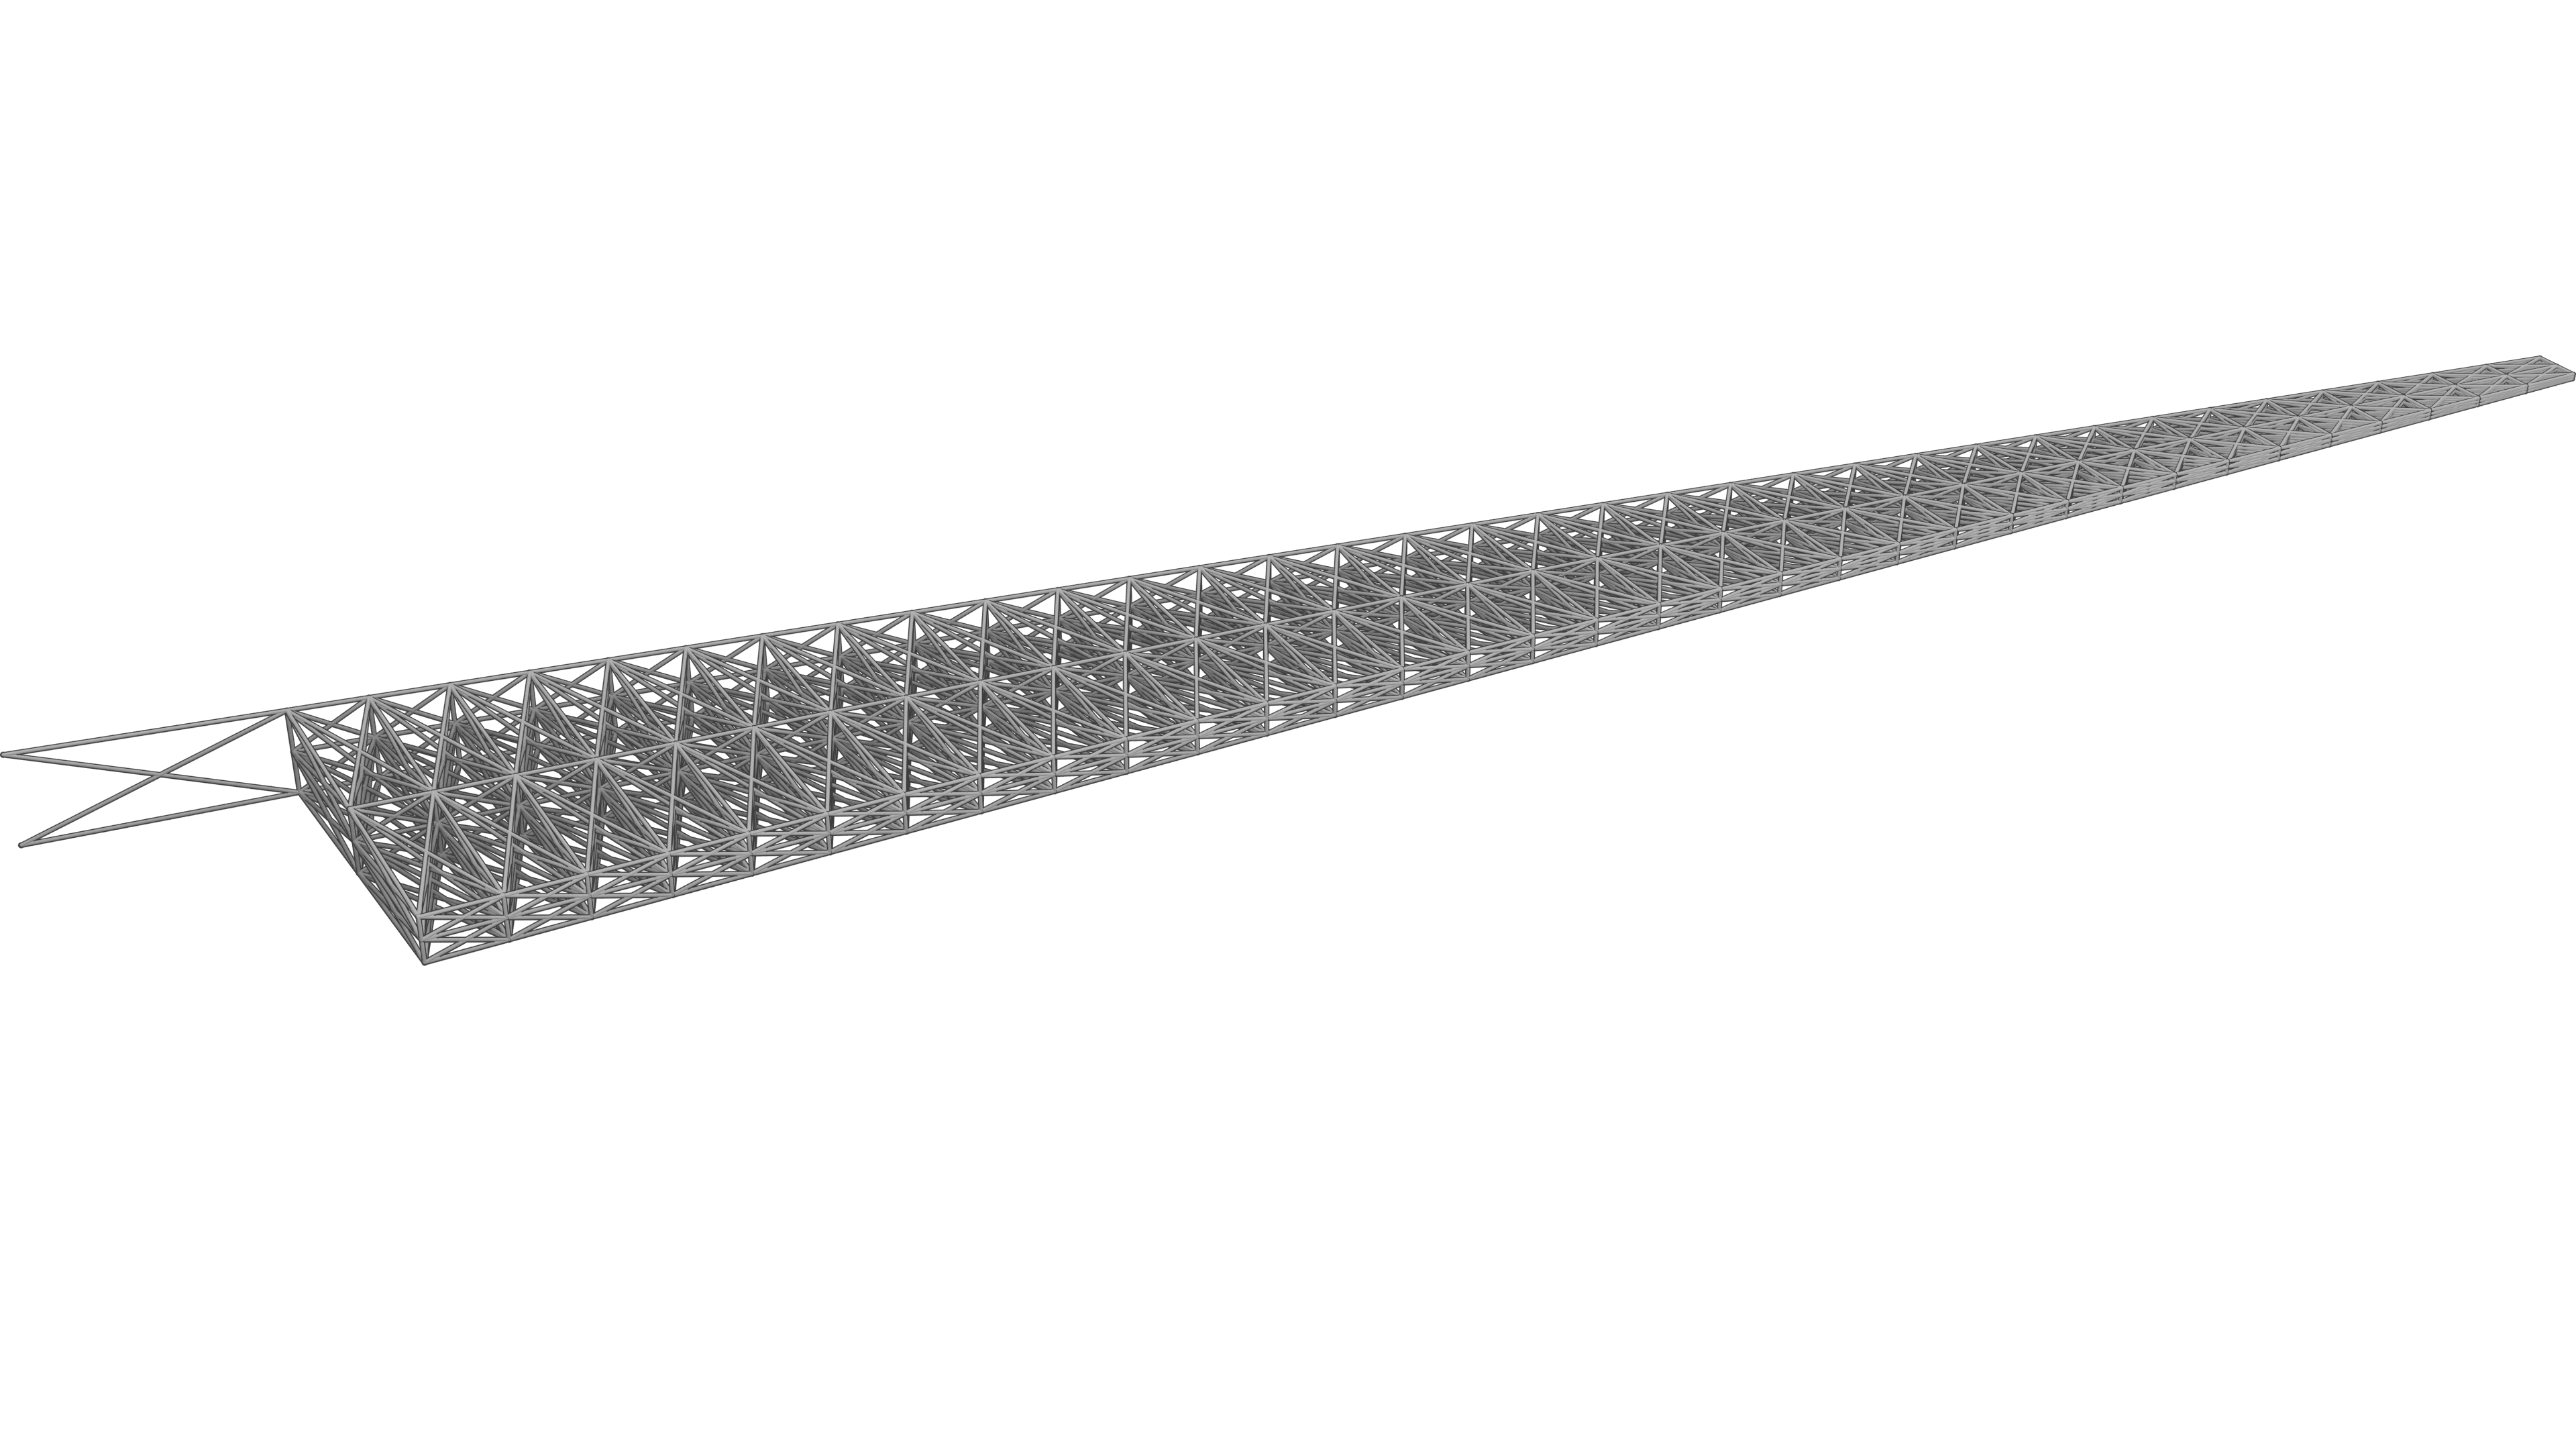
\includegraphics[width=0.45\linewidth]{figures/07_aeronautic/14b_00_Topology_x0_iso 2370.png}}
        \caption{(a) Ground structure of the CRM-315 test case; (b) Ground structure of the CRM-2370 test case. The cross-sectional areas shown in the two sub-figures represent the starting point of the optimizations.}
        \label{fig:07_crm}
    \end{figure*}
    
    \begin{figure}
        \centering
        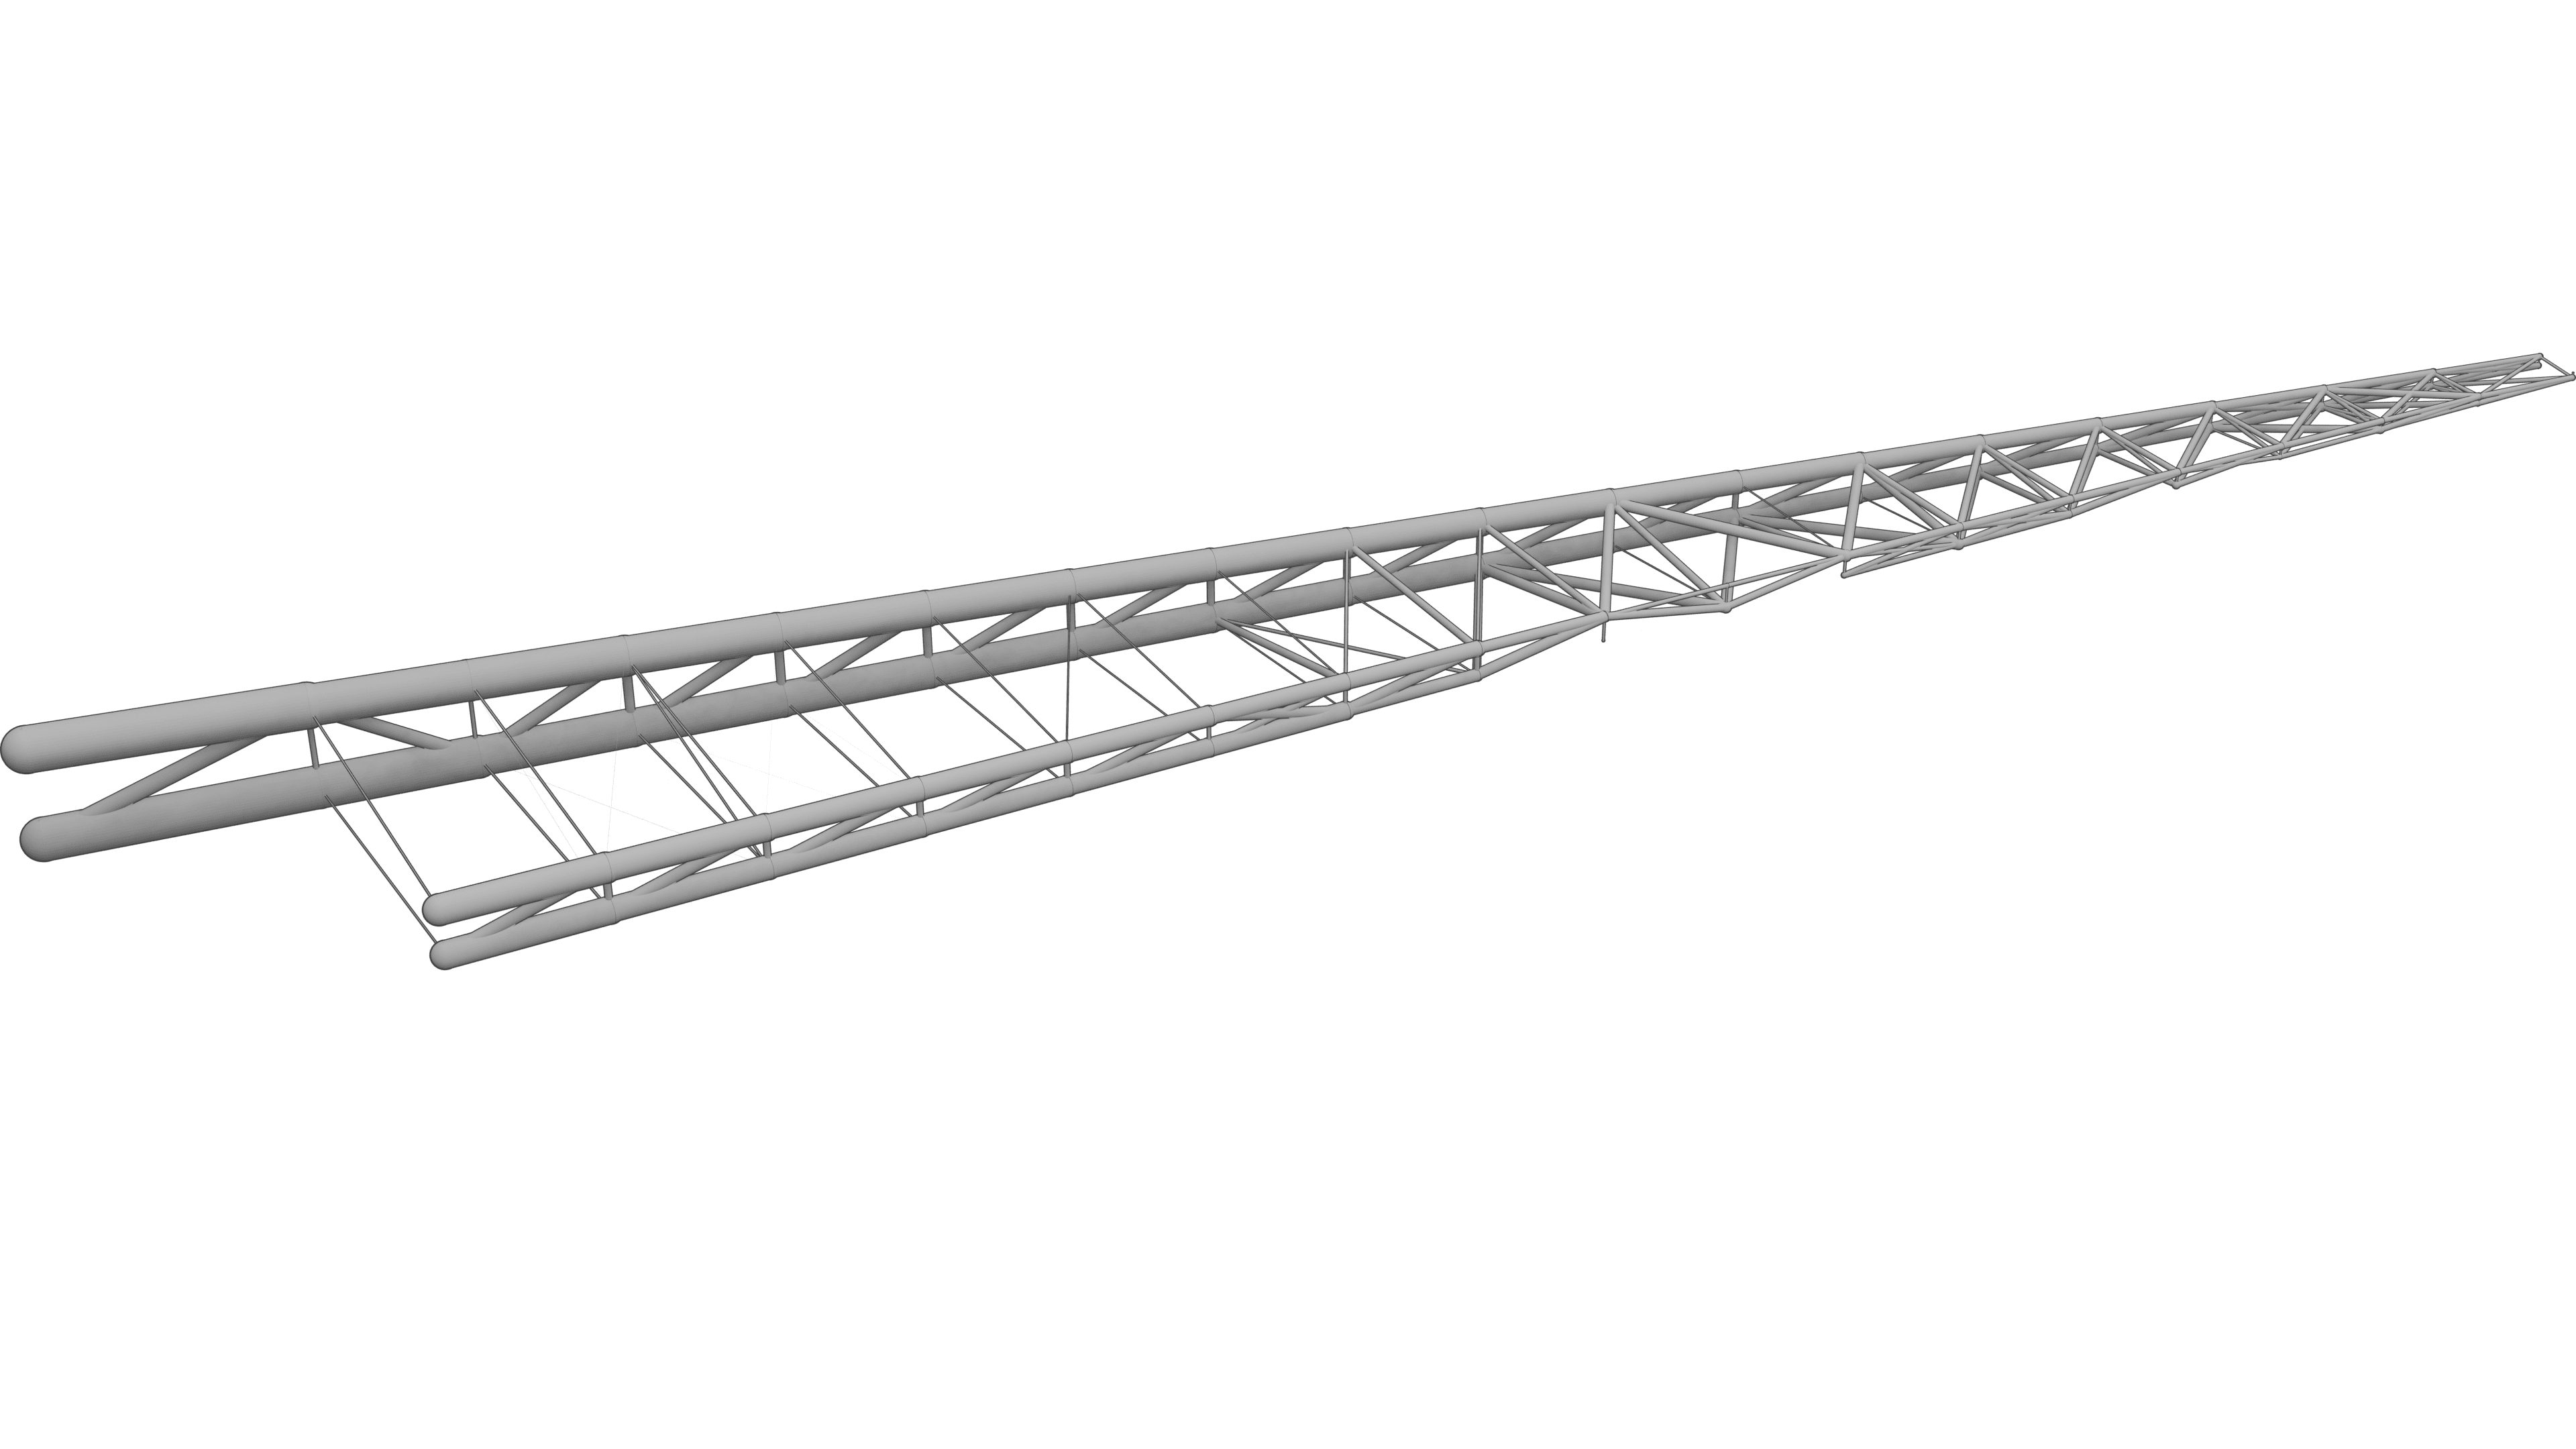
\includegraphics[width=0.8\linewidth]{figures/07_aeronautic/15_04_Topology_NLP_iso.png}
         \caption{Optimized topology of the CRM-315 with 257 active bars.}
        \label{fig:07_crm315}
    \end{figure}
    
    Two different discretization schemes are considered for the optimization. The proposed algorithm is firstly tested on the same ground structure provided by Fakhimi \etal \sidecite{fakhimi_discrete_2021}, composed of $N_{\text{el}}=315$ candidate members (CRM-315). The second discretization is obtained by refining the 315-bar ground structure, evaluating the midpoints of every member, and connecting them with first-order connectivity. We obtain $N_{\text{el}}=2370$ candidate members (CRM-2370). The loads and the boundary conditions are applied on the same nodes of the ground structure for the two studied ground structures. The cross-sectional areas of the starting point of the CRM-315 and the CRM-2370 are set to \qty{0.0001}{m^2} and they are shown in \figref{fig:07_crm}. Only one single starting point is used for these two examples as \chpref{chap:04} demonstrated that the proposed two-step strategy with reinitialization reduces the reliance of the optimization result on the starting point. The resolution algorithm used is 2S-5R. The numerical results of the optimization for the two different discretizations are reported in \tabref{tab:07_wing-res}. 
    
    The optimized CRM-315 structure shows a mass of \qty{21.342}{\tonne}, a \qty{27.01}{\%} reduction compared to the solution with discrete cross-section areas found by Fakhimi \etal \sidecite{fakhimi_discrete_2021} (\qty{29.238}{\tonne}). Other than the substantial difference in the modelization of the cross-section areas\sidenote{It is to be reminded that Fakhimi \etal constrained the optimization problem to utilize only discretized values for the cross-sectional areas.}, the mass reduction could be explained by the fact that the proposed algorithm allows members to vanish: the 2S-5R solution shows 257 active bars out of 315 at convergence (see \figref{fig:07_crm315}). In contrast, the \gls{milo} problem solved by Fakhimi \etal \cite{fakhimi_discrete_2021} is employed as a sizing optimization algorithm with fixed topology (and thus 315 active members in the optimized design). A more detailed comparison could not be performed as the authors did not share the values of the cross-sectional areas of their solution. 
    
    The volume fraction of the solution is \qty{1.313}{\percent} and the minimum slenderness ratio $\lambda$ (ratio between the length and the radius of gyration of the bar) of a bar is 14.96, which validates the choice of a truss model used to discretize the wingbox volume. The execution time of the optimization is \qty{19}{s} for the \gls{slp} step and \qty{128}{s} for the \gls{nlp} step, for a total of \qty{147}{s} on a regular notebook, compared to more than four days of optimization of Fakhimi \cite{fakhimi_discrete_2021} on a desktop workstation. The iteration history curves of the optimization are plotted in Figure \ref{fig:07_c2}a, where we notice the multiple sharp volume increases due to the reinitialization heuristic in the \gls{slp} step. Figure \ref{fig:07_c2}b, on the other hand, shows the constraint violation curves for the \gls{nlp} phase. The starting point coming from the relaxed \gls{slp} step violates the stress and buckling constraints as the predicted force field does not account for kinematic compatibility, necessary due to the multiple loading conditions of this test case. From the graph, we can observe how challenging it is to satisfy the kinematic compatibility constraint.

    \begin{table}
        \small
        \centering
        \begin{tabular}{ccc}
        \toprule
        \textbf{Quantity} & \textbf{CRM-315} & \textbf{CRM-2370} \\ \midrule
        N$_{\text{el}}$          & 315               & 2370               \\
        N$_{\text{opt}}$           & 257                  &  1127              \\
        V [\unit{\meter^3}]             &  7.90                 &  7.44             \\
        V [\unit{\%}]             &   \qty{1.309}{\%}                & \qty{1.232}{\%}               \\
        Mass [\unit{\tonne}]               &   21.342                & 20.092     \\
        a$_{\text{max}}$ [\unit{\meter^2}]           &  0.198                 & 0.208              \\
        C$_\text{LC\_1}$ [\unit{\mega \joule}]                &  3.23                 &  3.17              \\
        C$_\text{LC\_2}$ [\unit{\mega \joule}]                &   1.28                &  1.27              \\
        C$_\text{LC\_3}$ [\unit{\mega \joule}]                &   0.76                &  0.74              \\
        t [\unit{\second}]                & 147                  & 3189   \\ \bottomrule            
        \end{tabular}
        \caption{Numerical results of the optimization of the CRM with two different ground structures.}
        \label{tab:07_wing-res}
    \end{table}

    \begin{figure*}
        \centering
        \subcaptionbox{}{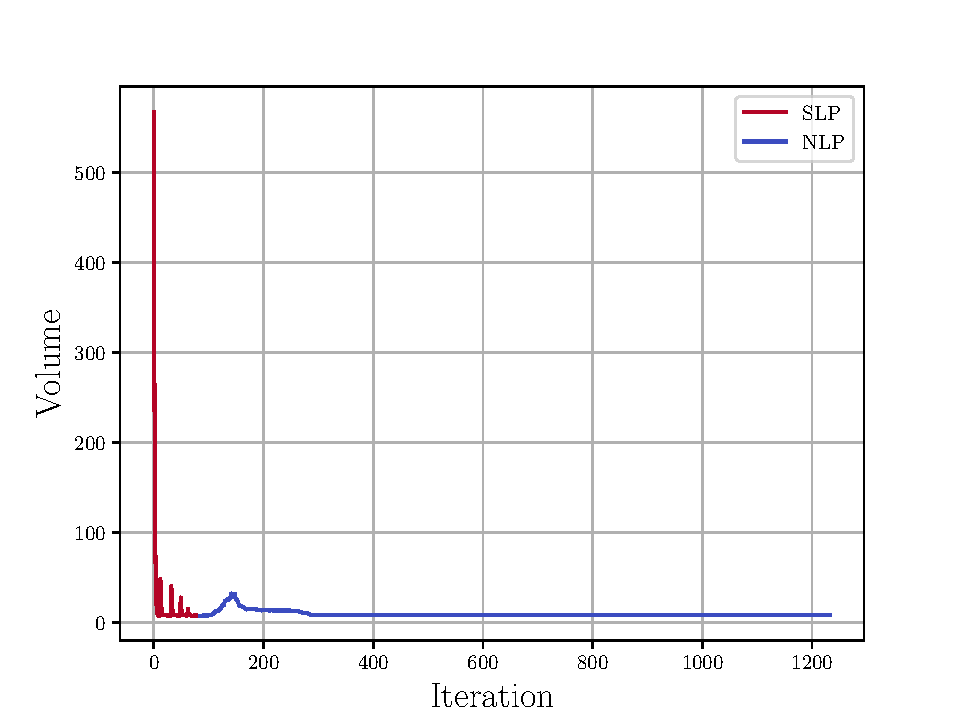
\includegraphics[width=0.45\linewidth]{figures/07_aeronautic/19a_v_hist_315.pdf}}
        \bigskip
        \subcaptionbox{}{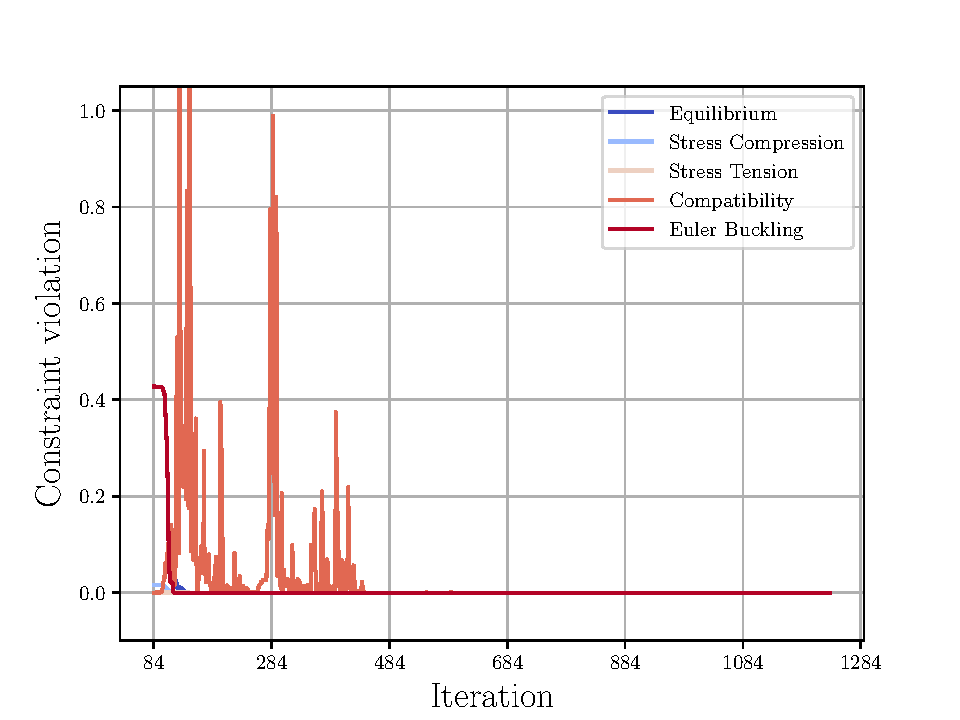
\includegraphics[width=0.45\linewidth]{figures/07_aeronautic/19b_c_hist_315.pdf}}
        \caption{Iteration history of the CRM-315 test case solved with the 2S-5R algorithm. (a) objective function history for the SLP and NLP step. The sharp increases in the objective function during the SLP step correspond to the reinitialization calls. (b) constraint violation for the NLP step.}
        \label{fig:07_c2}
    \end{figure*}

\paragraph{Maximum Displacement Constraints}
An aircraft designer may wish to restrict the maximum Z displacement of the wingtip $Z_{t,\ell}$ to prevent excessive bending of the wing, which could significantly affect the aerodynamic performance of the wing. It is important to note that by controlling the maximum displacements of the structure, we can effectively influence its compliance, even if compliance minimization is not explicitly included in the objective function. Additionally, imposing such constraints can passively enhance the stiffness of the wing and mitigate aeroelastic phenomena such as flutter instability.

Having observed that in the unconstrained version the maximum tip displacement of the optimized CRM-315 structure, which has a half wing span of \qty{29.4}{m}, is $Z_\text{t}=\qty{4.11}{m}$, we set three different maximum wingtip displacement values $Z_{t,\ell} = [\qty{1}{m},\qty{2}{m},\qty{3}{m}]$ in the \gls{nlp} step, intending to explore how sensitive the optimized structure is with respect to this constraint. These constraints are simply put as bound constraints on the displacement design variable in the \gls{nlp} step. The optimization runs are conducted using the same data (materials, geometry, load cases) as in the previous example.

\begin{table}
    \small
    \centering
    \begin{tabular}{ccccc}
    \toprule
    $\bm{Z}_{t,\ell}\:[\text{m}]$ & 1&2&3&--\\ \midrule
    V [\unit{\meter^3}]&  26.70&13.78&9.39&7.90\\
    V [\unit{\%}]&   \qty{4.421}{\%}   & \qty{2.283}{\%}&\qty{1.556}{\%}&\qty{1.309}{\%}  \\
    Mass [\unit{\tonne}]  &72.086&37.218&25.363&21.342\\
    a$_{\text{max}}$ [\unit{\meter^2}]&  0.615    & 0.293&0.197&0.198\\
    C$_\text{LC\_1}$ [\unit{\mega \joule}]   &  1.05    &  1.96&2.79& 3.23\\
    C$_\text{LC\_2}$ [\unit{\mega \joule}]   &   0.37   &  0.71&1.04& 1.28\\
    C$_\text{LC\_3}$ [\unit{\mega \joule}]   &   0.26   &  0.47&0.67& 0.76\\

    \bottomrule
    \end{tabular}
    \caption{Numerical results of the optimization of the CRM-315 model with three different maximum displacement constraints ($Z_{t,\ell}=\qty{1}{m}$, $Z_{t,\ell}=\qty{2}{m}$, $Z_{t,\ell}=\qty{3}{m}$) and no maximum displacement constraints.}
    \label{tab:07_disp}
\end{table}

\begin{figure*}
    \centering
    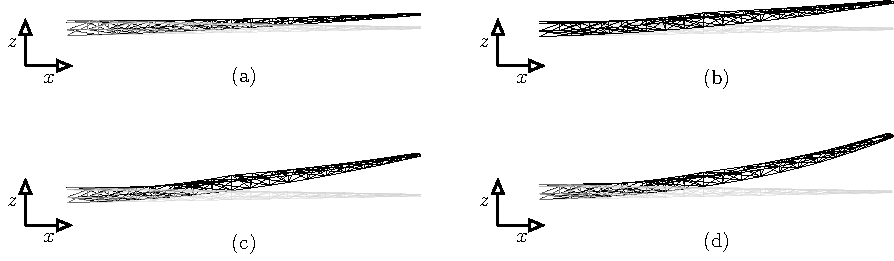
\includegraphics[width=\linewidth]{figures/07_aeronautic/00_dispalcements/disp.pdf}
     \caption{Undeformed (gray) and deformed (black) shapes of the optimized CRM-315 structures with a half wing span of \qty{29.4}{m} for different values of maximum Z displacement $Z_{t,\ell}$ of the wing tip constraints for the LC\_1 load case. (a) $Z_{t,\ell}=\qty{1}{m}$  ; (b) $Z_{t,\ell}=\qty{2}{m}$; (c) $Z_{t,\ell}=\qty{3}{m}$; (d) no maximum displacement constraints.}
    \label{fig:07_disp_sol}
\end{figure*}

We run the three additional optimizations and we plot the displacements in the XZ plane in \figref{fig:07_disp_sol} and the numerical values of the optimization in \tabref{tab:07_disp}. Firstly, we notice how effectively the optimizer limited the maximum displacement and converged to a solution even with a hard-to-satisfy constraint such as $Z_{t,\ell}=\qty{1}{m}$ \marginnote{We note that the \gls{crm} has a half wing span of \qty{29.4}{m}.}. Secondly, we observe that this positive result is not without drawbacks. Indeed, the added rigidity needed to comply with the maximum displacement constraint comes from a significant weight gain, representing a \qty{19}{\percent}, \qty{75}{\percent}, and \qty{237}{\percent} increase compared to the unconstrained case for $Z_{t,\ell} = [\qty{3}{m},\qty{2}{m},\qty{1}{m}]$, respectively. Finally, as already mentioned, the constraints on maximum displacements significantly influence the compliance of the structure. Having a further look at \tabref{tab:07_disp}, it becomes apparent that the compliance decreases as the displacement constraints become more restrictive. This observation implies that even though the formulation proposed does not explicitly address compliance, it can still be indirectly influenced by adjusting these constraints.

\paragraph{Multiple materials}
The proposed formulation uses material data as input for the optimization, and until this point, we have not investigated how material data could influence the topology and the final volume of the optimized structure. However, we recognize the importance of the choice of material properties, and here, we aim to examine their influence on the CRM-315 test case.

\begin{table}
    \small
    \centering
    \begin{tabular}{ccccc}
    \toprule
    \textbf{Material} &\textbf{Aluminium}&\textbf{Titanium}&\textbf{Steel}&\textbf{Pultruted CFRP}\\ \midrule
    $E$& \qty{69}{GPa}&\qty{120}{GPa}&\qty{210}{GPa}&\qty{150}{GPa}     \\
    $\sigma_\text{c}, \sigma_\text{t}$ & $\pm $\qty{270}{MPa}&$\pm $\qty{880}{MPa}&$\pm $\qty{355}{MPa}&+1200,\qty{-880}{MPa} \\
    $\rho$& \qty{2.7}{\gram\per\cubic\centi\metre}&\qty{4.5}{\gram\per\cubic\centi\metre}&\qty{7.8}{\gram\per\cubic\centi\metre}&\qty{1.6}{\gram\per\cubic\centi\metre}   \\
    \unit{kg CO_2^{\text{eq}}\per\kilo\gram}&12.5&47.0&5.0&34.5 \\
    \unit{\$\per\kilo\gram}&2.2&23.5&6.3&40.5\\
    \bottomrule
    \end{tabular}
    \caption{Material data of the four materials used for the CRM-315 optimization.}
    \label{tab:07_materials_data}
\end{table}

We use four different materials commonly used in the aerospace domain: an aluminum alloy, titanium alloy, stainless steel, and pultruded \gls{cfrp}, each with mechanical properties as reported in \tabref{tab:07_materials_data}. In addition to classic material properties such as Young's modulus, yield stress, and density, we also considered the environmental cost \unit{CO^{eq}_2}, \ie, the mass of equivalent CO$_2$ emitted to produce a unit mass of the material, as well as the economic cost in dollars. These values were sourced from Ashby's book \sidecite{ashby_materials_1999}.

\begin{table}
    \small
    \centering
    \begin{tabular}{ccccc}
    \toprule
    \textbf{Material} &\textbf{Aluminium}&\textbf{Titanium}&\textbf{Steel}&\textbf{Pultruted CFRP}\\ \midrule
    V [\unit{\meter^3}]&7.90&4.53&5.88&3.67\\
    V [\unit{\%}]&\qty{1.309}{\%}&\qty{0.749}{\%}&\qty{0.974}{\%}&\qty{0.607}{\%}\\
    Mass [\unit{\tonne}]& 21.342&20.372&46.168&5.868\\
    a$_{\text{max}}$ [\unit{\meter^2}]&0.198&0.088&0.153&0.086\\
    C$_\text{LC\_1}$ [\unit{\mega \joule}]&3.23&4.88&1.33&4.39\\
    C$_\text{LC\_2}$ [\unit{\mega \joule}]&1.28&1.94&0.53&1.73\\
    C$_\text{LC\_3}$ [\unit{\mega \joule}]&0.76&1.15&0.31&1.03\\
    $Z_\text{t}\:[\text{m}]$&4.10&5.97&1.70&5.31\\
    Cost [\unit{\tonne CO_2^{\text{eq}}}]&266.7&957.5&230.8&202.4\\
    Cost [\unit{k\$}]&46.9&478.7&290.8&237.6\\
    \bottomrule
    \end{tabular}
    \caption{Numerical results of the CRM-315 optimized using four different materials.}
    \label{tab:07_materials}
\end{table}

The numerical results of the optimizations are presented in \tabref{tab:07_materials}, and several observations can be made. First, we confirm that the mass of the optimized structure is highly influenced by the choice of material, particularly by the specific resistance ($\sigma_\text{L}/\rho$) and specific stiffness ($E/\rho$) of the material. Second, we notice that the values of compliance $C$ and maximum tip displacement $Z_\text{t}$ are also greatly influenced by material data, specifically by the ratio between strength and Young's modulus of the material ($\sigma_\text{L}/E$). This is because a stronger material leads to smaller cross-sectional areas and thus lower global stiffness. While these observations may seem trivial, it was nonetheless important to verify that the optimizations yield the expected trends. Third, the volume behavior follows a hyperbolic law with respect to the strength of the material, as in this specific case, the most voluminous elements are constrained by stress rather than buckling (see the constraints' analysis at page~\pageref{sec:07_amc}). Finally, we present the deformed structures in \figref{fig:07_mat_sol}, which strongly highlights the highly deformed shapes obtained with titanium and pultruded CFRP, due to their superior resistance properties. 

We then observe the environmental and economic cost of the four structures. Upon inspection of \figref{fig:07_cost}, we notice that, apart from titanium, the structures exhibit almost the same environmental cost for material production. This is unexpected given the significantly different specific CO$_2$ emissions of the four materials; for instance, there is nearly a seven-fold difference between steel and CFRP. However, the CFRP solution demonstrates a massive weight reduction, ultimately favoring it over steel and even aluminum. A similar trend is observed in terms of cost, although the very low production cost favors aluminum over all other materials. It appears that, for this specific load case, CFRP, despite costing more than aluminum, represents the best compromise between excellent mechanical properties, environmental impact, and economic cost. Finally, it should be noted that here we only considered the material cost, but the lower weight on an aircraft leads to much greater savings compared to the cost of material production alone. This further favors the pultruded CFRP solution.

\begin{figure*}
    \centering
    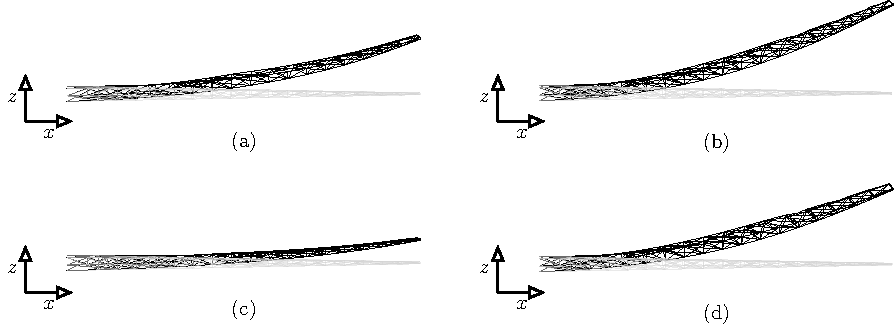
\includegraphics[width=\linewidth]{figures/07_aeronautic/00_materials/mat.pdf}
     \caption{Undeformed (gray) and deformed (black) shapes of the optimized CRM-315 structures with four different materials for the LC\_1 load case; (a) aluminum with $Z_\text{t}=\qty{4.10}{m}$; (b) titanium with $Z_\text{t}=\qty{5.97}{m}$; (c) stainless steel with $Z_\text{t}=\qty{1.70}{m}$; (d) pultruded CFRP with $Z_\text{t}=\qty{5.31}{m}$.}
    \label{fig:07_mat_sol}
\end{figure*}

\begin{marginfigure}
    \centering
    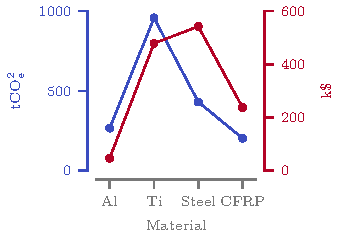
\includegraphics[width=\linewidth]{figures/07_aeronautic/00_co2eq/co2_dollar.pdf}
    \caption{Environmental and economic cost of the CRM-315 structure optimized using four different materials: aluminum, titanium, stainless steel, and pultruded CFRP.}
    \label{fig:07_cost}
\end{marginfigure}

\paragraph{Enriching the mesh}
As described earlier in the chapter, we now aim to assess the influence of the initial ground structure on the volume and topology of the optimized structure. Thus, the same optimization is performed on a refined ground structure, referred to as CRM-2370, with aluminum as the material.
\begin{figure*}
    \centering
    \includegraphics[width=1\linewidth]{figures/07_aeronautic/16_wing_opt/wing_opt.pdf}
     \caption{Maximum stress constraint value (left) and buckling constraint value (right) plotted on the deformed shape of the optimized design (undeformed shape in light grey) of CRM-2370 for the three load cases: +2.5 g maneuver (a), -1 g maneuver (b), and cruise with gust (+1.3 g) (c). The maximum $z$ tip deflection is \qty{4.167}{m}, \qty{-2.953}{m}, and \qty{1.948}{m}, respectively.}
    \label{fig:07_wing_opt}
\end{figure*}

The mass of the optimized CRM-2370 structure is \qty{20.092}{\tonne}, a \qty{1.318}{\tonne} reduction compared to the CRM-315 (\qty{-6.2}{\%}). Additionally, if we compare the compliance of the three load cases (see \tabref{tab:07_wing-res}), we notice how the solution of CRM-2370 is not only lighter but also stiffer, suggesting in general a more efficient structure topology. The maximum tip deflection of the wingbox $Z_\text{t}$ is \qty{4.167}{m}, \qty{-2.953}{m}, \qty{1.948}{m} for the three considered load cases, respectively. There are 1127 active bars in the optimized design, and the whole optimization took \qty{3189}{s} (\qty{1911}{s} for the \gls{slp} step, \qty{1278}{s} for the \gls{nlp} step). The iteration history curves of the optimization are plotted in \figref{fig:07_c3}. In \figref{fig:07_wing_opt} the normalized maximum stress and buckling constraints are plotted on the deformed shape of the three load cases. We notice how in general the topology of the two external "spars" is shaped after the +2.5 g load case, while the interior of the wingbox is made by a thinner truss constrained by buckling. 

\begin{figure*}
    \centering
    \subcaptionbox{}{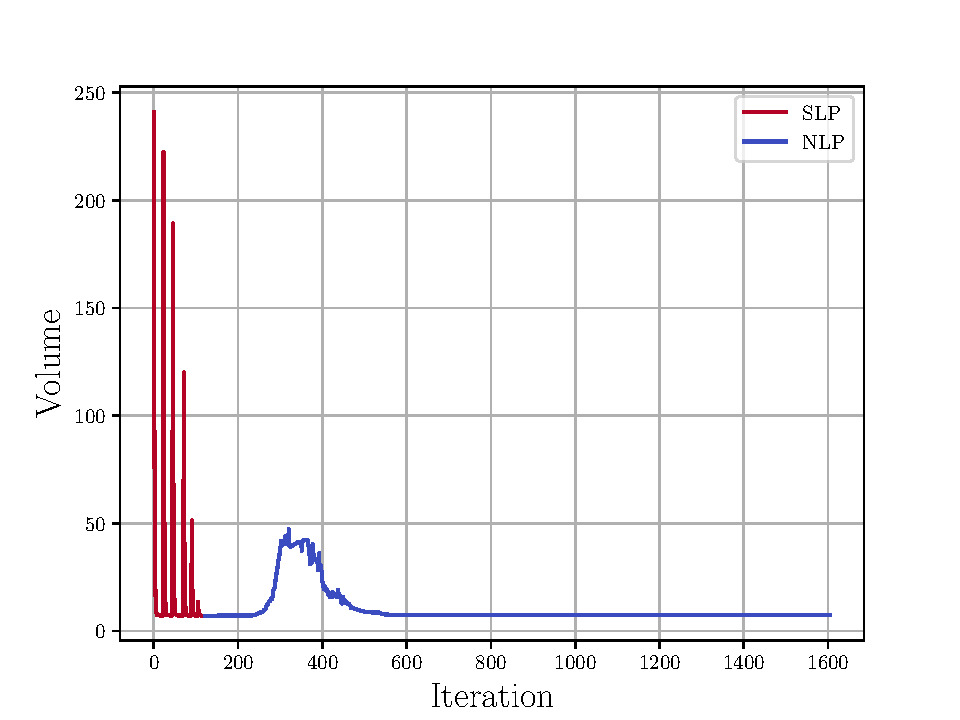
\includegraphics[width=0.45\linewidth]{figures/07_aeronautic/20a_v_hist_2370.pdf}}
    \bigskip
    \subcaptionbox{}{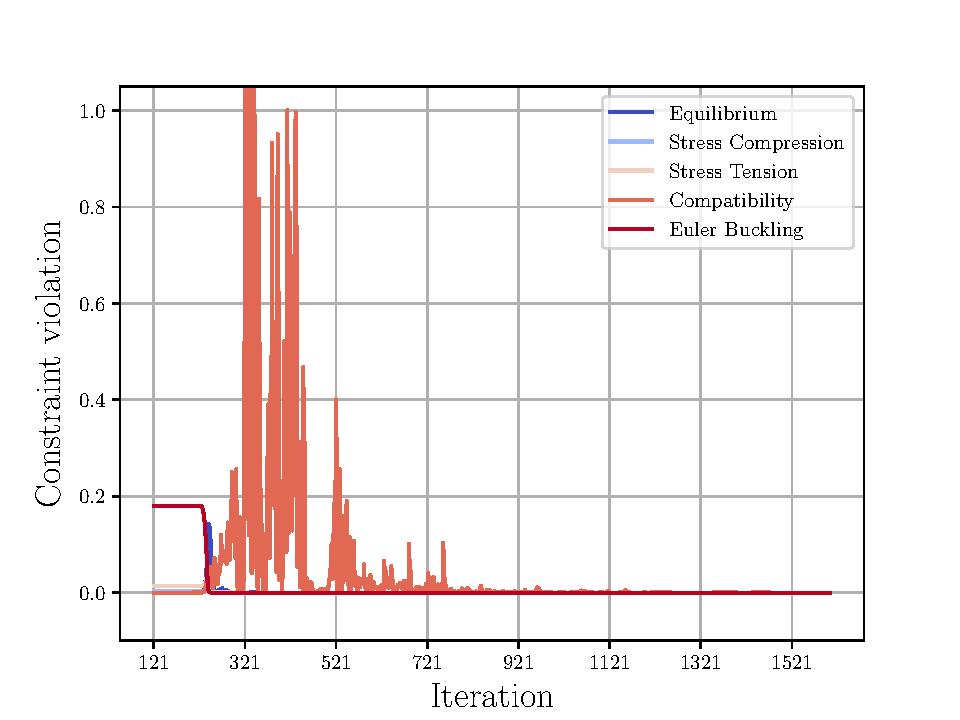
\includegraphics[width=0.45\linewidth]{figures/07_aeronautic/20b_c_hist_2370.pdf}}
    \caption{Iteration history of the CRM-2370 example solved with the 2S-5R algorithm. (a) objective function history for the SLP and NLP step. The sharp increases in the objective function during the SLP step correspond to the reinitialization calls. (b) constraint violation for the NLP step.}
    \label{fig:07_c3}
\end{figure*}

\FloatBarrier
\paragraph{Active mechanical constraints} \label{sec:07_amc}
\figref{fig:fail-crm} shows a scatter plot of the normalized buckling criterion $\vect{c}_\text{b}$ plotted against the normalized stress criterion $\vect{c}_\text{s}$, defined as follows:
\begin{equation}
    \vect{c}_\text{b}=\frac{\vect{q}\; \textit{\textbf{sf}}}{\vect{q}_{\text{crit}}},
\end{equation}
\begin{equation}
    \vect{c}_\text{s}=\max{\left(-\frac{\vect{q} \; \textit{\textbf{sf}}}{\sigma_c \vect{a}},\frac{\vect{q} \; \textit{\textbf{sf}}}{\sigma_t \vect{a}}\right)},
\end{equation}
Every point in the scatter plot represents a member of the \gls{slp} and the \gls{nlp} solutions. Only the active members are shown (931 out of 1127 members), \ie, members carrying a load superior to \qty{1}{N}. The reason is that the stress and buckling criteria are only evaluated on these members to avoid numerical issues that could occur for very small cross-section areas. All the \gls{slp} members activate either the maximum stress or buckling limit, while 68 out of 931 \gls{nlp} members are located in the center of the graph ($c_\text{s}<0.95$ and $c_\text{b}<0.95$). We speculate that this behavior is due to the inclusion of the kinematic compatibility constraint in the \gls{nlp} algorithm: the cross-sectional area of these bars is chosen to comply with the global displacements rather than the aforementioned criteria. In \tabref{tab:07_constrNLP} we present a summary of the active mechanical failure constraints (buckling, tensile stress, and compressive stress) present in the NLP solution. The table showcases the number of active constraints categorized by constraint type and load case. The optimized design encompasses a total of 930 active mechanical failure constraints for 863 bars (931 minus the 68 bars constrained by kinematic compatibility). This suggests that certain members are concurrently subject to multiple failure constraints across different load cases. An additional observation is that the design of the solution is primarily influenced by local buckling and compressive failures, especially under the +2.5 g load case (LC\_1).

\begin{figure}
    \centering
    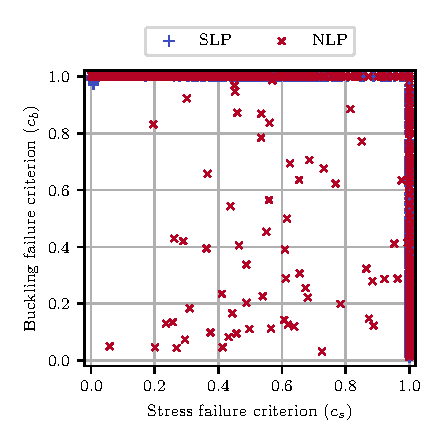
\includegraphics[width=0.8\linewidth]{figures/07_aeronautic/18_failure new/failure_max.pdf}
     \caption{Normalized buckling and maximum stress constraint values for the optimized CRM-2370 structure after the SLP and the NLP optimization steps.}
    \label{fig:fail-crm}
\end{figure}

\begin{table}
\small
\centering
\begin{tabular}{lS[table-format=3.0]S[table-format=3.0]S[table-format=3.0]S[table-format=3.0]S[table-format=3.0]}
\toprule
                     & \textbf{LC\_1} & \textbf{LC\_2} & \textbf{LC\_3} & \textbf{Tot.} \\ \midrule
\textbf{Buckling}    & 281           & 145           & 143           & 569           \\
\textbf{Tension}     & 56            & 3             & 4             & 63            \\
\textbf{Compression} & 286           & 6             & 6             & 298           \\
\midrule
\textbf{Tot.}        & 623           & 154           & 153           & 930          \\
\bottomrule
\end{tabular}
\caption{Number of active mechanical failure constraints for the CRM-2370 optimized design per type of constraint (rows) and per load case (columns).}
\label{tab:07_constrNLP}
\end{table}

\paragraph{Discussion on the modular CRM}
The analysis of the optimization of the monolithic \gls{crm} wingbox is now complete, and we are considering utilizing the modular algorithm presented in \chpref{chap:06}. However, this particular test case presents significant challenges if we opt for modular optimization. The high elongation along the X-axis and the tapered chord and thickness of the wingbox make it difficult to conceive a modular ground structure. One potential approach, similar to that used by Cramer \etal \sidecite{cramer_elastic_2019}, subdivides the volumetric domain of the wing into modular and "filler" domains, with the filler serving to connect the external shape to the modular part. However, this method may not be efficient for this specific case due to the need for excessively small modules, increasing computational costs, or resulting in a high ratio of filler volume to modular volume. Moreover, structures of this size may not benefit as much from some modular advantages, such as ease of field deployment.

For these reasons, we decided to switch to a smaller but still very relevant test case. We turn our attention to another aeronautical application. One of the most suitable applications for modular structures is their use in small fixed-wing \glspl{uav}. This is due to their inherent ease of field deployment, ease of repair and transport, and the extremely lightweight properties of modular lattice structures.

\section{NACA 0012 modular UAV wing} \label{sec:07_wing}
\begin{margintable}
    \small
    \centering
    \begin{tabular}{cc}
    \toprule
    \textbf{Parameter}        & \textbf{Value} \\ \midrule
    $E$              & \qty{6.8}{GPa}     \\
    $\sigma_\text{c}, \sigma_\text{t}$ & $\pm $\qty{140}{MPa} \\
    $\rho$              & \qty{1.42}{\gram\per\cubic\centi\metre}   \\
    \bottomrule
    \end{tabular}
    \caption{Material data of the Ultem 2200 used for the NACA 0012 optimization.}
    \label{tab:07_NACA_mat}
\end{margintable}
\begin{figure}
    \centering
    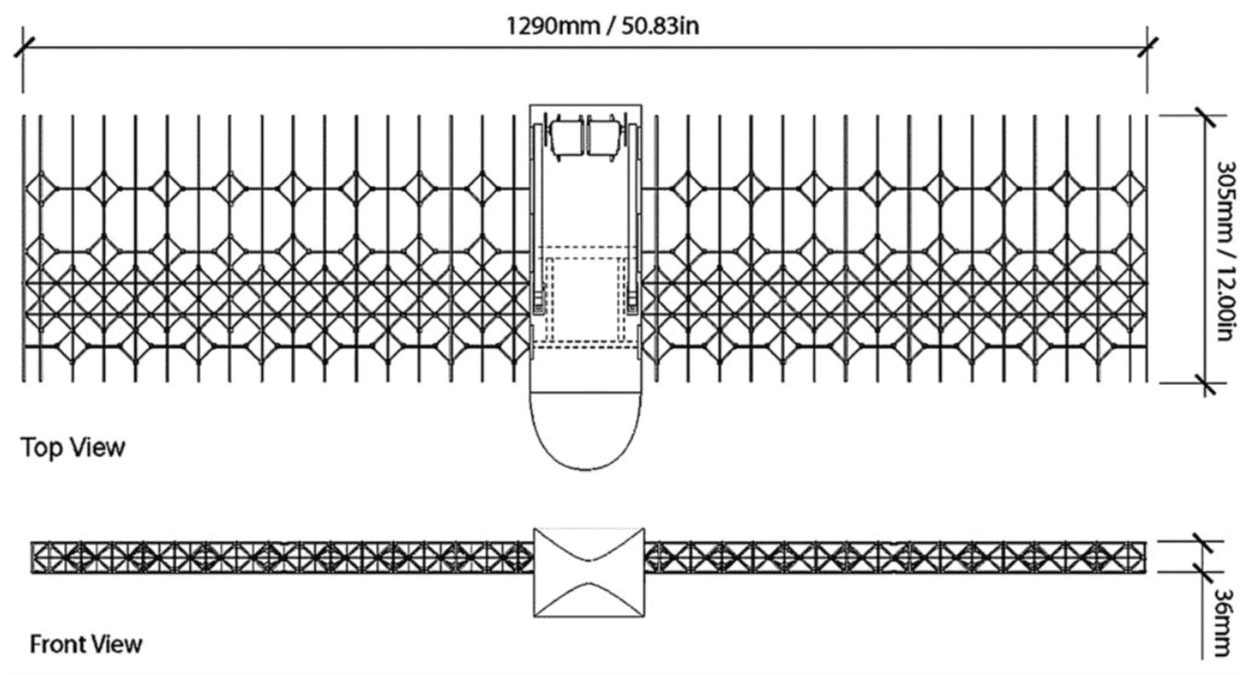
\includegraphics[width=0.8\linewidth]{figures/07_aeronautic/naca0012.png}
        \caption{The Digital Morphing Wing Platform developed at NASA \cite{jenett_digital_2017}.}
    \label{fig:07_naca0012}
\end{figure}
Jenett and his working group at NASA developed an experimental platform for studying active morphing wings using lattices, the dimensions of which are shown in Figure \ref{fig:07_naca0012}. The wing volumetric domain for this platform is obtained by extruding a NACA 0012 airfoil with a chord of $c=\qty{305}{mm}$ by a span of $b=\qty{580}{mm}$. For our modular optimization, we adopt the same volumetric domain and focus on optimizing the internal structure for static loading rather than focusing on the aerodynamic properties of the profile and aeroelastic objectives and constraints (flutter, divergence). As the platform was not designed for flight, additional data on the internal structure requirements is not provided by the authors. Therefore, we conservatively assume a maximum takeoff weight of $\text{MTOW}=\qty{10}{kg}$ and design the structure to withstand a maximum loading factor of $\text{nz}=2$. The wing has a rectangular planform on the XY plane, and we assume a constant lift distribution along the X-axis (span of the extruded profile). Additionally, we simplify by assuming the lift distribution is constant along the Y-plane (chord plane). The lift distribution is then integrated to evaluate the concentrated nodal loads required for our optimization. In this setup, all nodes on the upper skin are equally loaded in the Z-direction. Similar to the CRM test case, we neglect the effect of the skin on the mechanical model. The wing is fixed at the root ($X=0$). Finally, we employ Ultem 2200 as the material for optimization, a high-performance thermoplastic material filled with \qty{20}{\percent} glass fiber, known for its strength and heat resistance. The mechanical properties are summarized in Table \ref{tab:07_NACA_mat}.

\subsection{Modular ground structure generation for irregular volumes}
Compared to the academic test cases presented in \chpref{chap:05} and \chpref{chap:06}, the extruded NACA 0012 profile does not have a regular parallelepipedal volume that can be easily partitioned into cubic subdomains. The simplest solution in this scenario would be to partition the structure into identical parts by performing multiple cuts on the YZ plane. However, this strategy may not apply to more complex volumetric domains. For this reason, we developed a ground structure generation strategy for complex, irregular volumes. It's important to note that for such structures, complete discretization using a parallelepipedal shape may not always be feasible. For instance, no matter how small we make a cubic module, we'll never be able to accurately discretize the curved shape of a sphere. Hence, the proposed strategy involves dividing the volumetric domain into two ground structures: one modular and the other serving as a filler for the non-modular regions. The primary objective of this strategy is to generate a modular ground structure for complex volumetric domains by maximizing the proportion of the modular part, thereby minimizing the filler volume.

To do so, we first generate a cloud of nodes equally distributed in the three axes in the bounding box of the volumetric domain we want to discretize. The distance between every node is chosen for all three axes and can be used as a hyperparameter that will define the size of the repeating module. Then, the points are tested for their position inside the volumetric domain using a winding number algorithm. This algorithm determines whether a point is inside or outside a volume by counting the number of times a ray from the point crosses the volume boundary. If the winding number is non-zero, the point is inside the volume; otherwise, it is outside. The points that are inside the volumetric domain are grouped into sets of eight and used as vertices of the parallelepipedal subdomains of the structure. At this point, additional equispaced nodes are added inside the newly generated subdomains according to the chosen module complexity\marginnote{Remember, we define module complexity as the number of nodes used to generate the modules' ground structure.}. This process results in a modular subdivision of a complex volume, minimizing the filler volume. This process is illustrated in the top row of \figref{fig:07_howto}.

Once the subdomains and additional nodes have been identified within the structure, a fully connected ground structure is built for every subdomain. The Delaunay triangulation algorithm is used instead to generate the ground structure for the filler volume. This algorithm uses the edges of the generated tetrahedra as members of the ground structure. The role of the filler ground structure is to transfer loads from the external boundary to the modular structure, and it can be optimized concurrently with the modular structure. Since the Delaunay triangulation algorithm uses the nodes of the modular ground structure as seeds for the mesh generation, the two discretizations are conformal. The final ground structure is obtained by superimposing the two discretizations, ensuring that the members of the filler part lying on the faces of the modular part are removed beforehand. An example of the generation of the two conformal discretizations is shown in the bottom row of \figref{fig:07_howto}.

\begin{figure*}
    \centering
    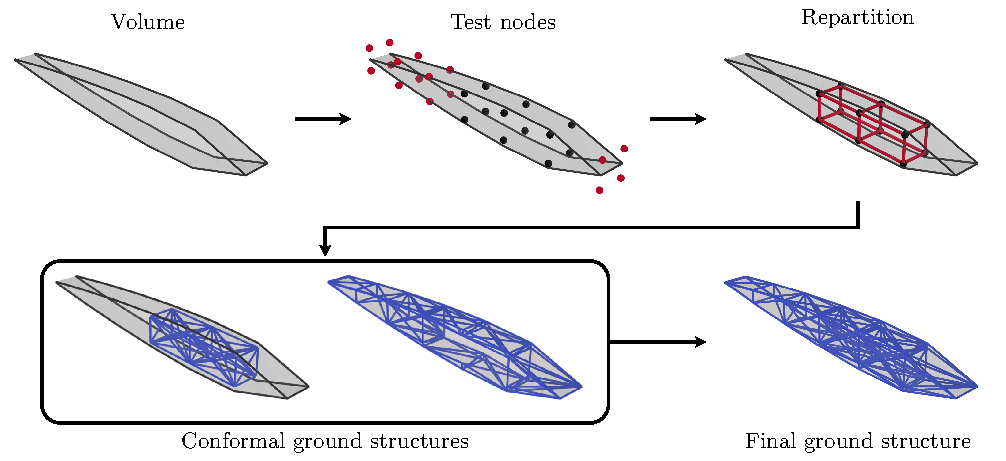
\includegraphics[width=\linewidth]{figures/07_aeronautic/00_naca_howtomesh/MESH.pdf}
     \caption{Ground structure generation flow chart of the proposed algorithm used to discretize irregular volumes and maximize the modular part.}
    \label{fig:07_howto}
\end{figure*}

\subsection{Numerical optimization of the modular NACA 0012 \gls{uav} wing}
The algorithm described above is utilized to generate the ground structure used for optimizing the modular NACA 0012 \gls{uav} wing. The volumetric domain of the wing is illustrated in \figref{fig:07_gs_a_types}a, together with the boundary conditions of the test case. In the case of the NACA 0012 wing, the filler part is very regular due to the extruded nature of the wing volumetric domain. Therefore, the Delaunay triangulation algorithm can easily output a modular ground structure for the filler volume as well. In this example, we define, thus, two different module types\sidenote{When referring to different module types, we are discussing distinct module external geometries and their corresponding bar connectivity configurations.}: the internal structure of the wing profile, referred to as the wingbox type, as it acts as the wingbox of the wing and is made up of parallelepipedic-shaped subdomains, and the profile type, which subdivides the original volume into wing sections that fill the space between the wingbox and the aerodynamic profile.

The parameters used to generate the modular ground structure are described here. The inter-distance between cloud points used for the wingbox-type ground structure generation is chosen in such a manner as to obtain 10 subdomains on the X-axis, 1 on Y, and 1 on Z. Each subdomain is made up of 2x2x2 nodes and a fully connected ground structure, totaling 28 candidate elements per module. Concerning the profile-type module, the extruded volume is divided into 5, 1, and 1 subdomains on the X, Y, and Z axes, respectively. Each module has a total of 175 candidates per module. A graphical representation of the two conformal ground structures is presented in \figref{fig:07_gs_a_types}b and \figref{fig:07_gs_a_types}c, while a comprehensive view of the full ground structure is shown in \figref{fig:07_gs_a}. This ground structure configuration is referred to as Configuration A.

\begin{figure*}
    \centering
    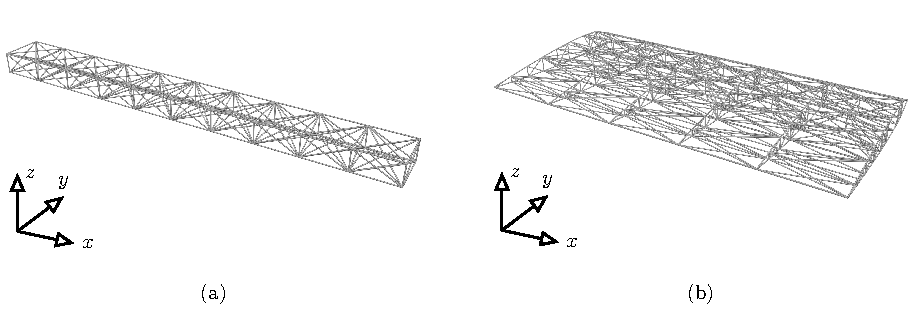
\includegraphics[width=\linewidth]{figures/07_aeronautic/00_NACA_a_gs_cell/gs_a_types.pdf}
     \caption{(a) Boundary conditions and volumetric domain of the NACA 0012 \gls{uav} wing; (b) wingbox type and (c) section type ground structures used for the optimization of the NACA 0012 \gls{uav} wing.}
    \label{fig:07_gs_a_types}
\end{figure*}

\begin{figure*}
    \centering
    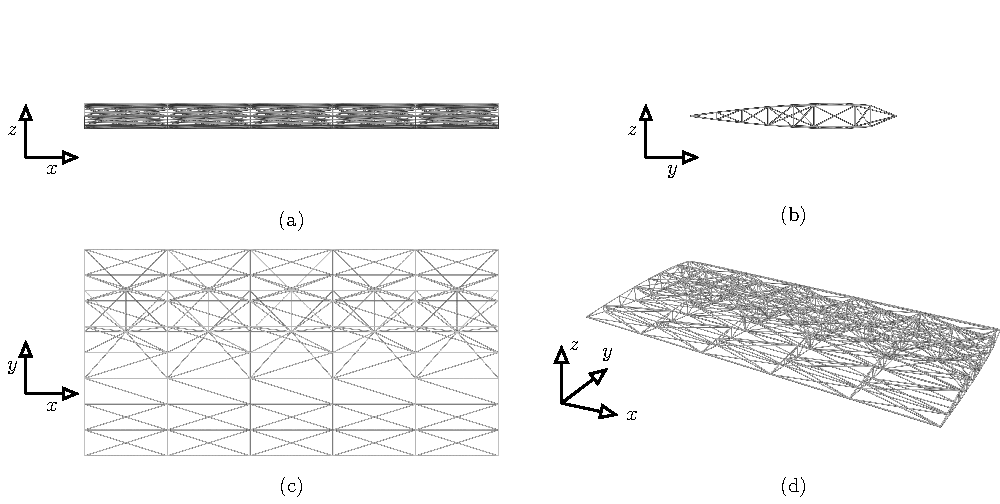
\includegraphics[width=\linewidth]{figures/07_aeronautic/00_NACA_gs/gs_a.pdf}
     \caption{Rendering of the complete ground structure used for the optimization of the NACA 0012 \gls{uav} wing seen from different viewing angles. This ground structure is formed by the superposition of two conformal ground structures: the wingbox and the section type.}
    \label{fig:07_gs_a}
\end{figure*}

The Configuration A ground structure is used to solve three different optimization problems. We set up all the problems using Ultem 2200 material and the wing dimensions, loading conditions, and boundary conditions described earlier in \secref{sec:07_wing}. The difference between each case lies in the use of a different number of module topologies $N_\text{T}$ for the three optimizations. We will start by analyzing the optimized structure behavior using a single topology $N_\text{T}=1$ for the two module types, and then we will increment to $N_\text{T}=2$ and $N_\text{T}=3$.

\begin{table*}
    \centering
    \small
    \begin{tabular}{lx{1.4cm}x{1.4cm}x{1.4cm}x{1.4cm}x{1.4cm}x{1.4cm}}
        \toprule
         &\multicolumn{3}{l}{Configuration A} & \multicolumn{3}{l}{Configuration B} \\ 
             \cmidrule(lr){2-4} \cmidrule(lr){5-7} 
    $N_\text{T}$&1&2&3&1&2&3\\
    $N_\text{opt}\;(N_\text{el})$ & 425 (1155)&503 (1155)& 366 (1155)&620 (1675)&539 (1675)&454 (1675) \\
    Mass [\unit{g}]&49.0&33.3&29.5&37.3&23.8&22.9 \\
    $V$ [\unit{\percent}] &0.81&0.55 &0.48&0.62&0.39&0.37        \\
    $\bar{\rho}$ [\unit{kg/m^3}] &11.53&7.84&6.93&8.76&5.59&5.38\\
    $\varphi$    &\qty{22.5}{\percent}&\qty{37.9}{\percent}&\qty{56.0}{\percent}&\qty{19.0}{\percent}&\qty{36.9}{\percent}&\qty{50.0}{\percent} \\
    $\psi$    &0.45&0.69&0.73&0.46&0.70&0.72\\ 
    t        & \hms{0;0;39}  & \hms{0;5;6} & \hms{0;2;3} & \hms{0;2;28} & \hms{0;3;32}&\hms{0;5;1}\\
    \bottomrule
    \end{tabular}
    \caption{Numeric results of the parametric study on the influence of the number of modules $N_\text{T}$ on the NACA 0012 \gls{uav} wing.}
    \label{tab:07_naca_num_res}
\end{table*}

\tabref{tab:07_naca_num_res} presents the numerical results of the optimization. Instead of reporting the volume, we focus on the mass and mass density in this table, as they are more easily understandable and have greater physical significance. In the columns corresponding to configuration A, we observe that the trends identified in \chpref{chap:06} persist: both the mass density and the mass of the structure decrease monotonically with the number of different module topologies, reaching a minimum of $M=\qty{29.5}{g}$ and $\bar{\rho}=\qty{6.93}{kg/m^3}$. This specific mass density $\bar{\rho}$ value is typical of aerogels \sidecite{ashby_materials_1999}, and comparable to values observed in NASA's MADCAT experimental platform \sidecite{cramer_elastic_2019}. Similar trends are evident in the performance parameters $\varphi$ and $\psi$, which tend towards \qty{100}{\percent} and $1.00$ respectively with the increase of $N_\text{T}$, indicating a more efficient use of the material in the solution. The number of active bars in the optimized solution, $N_\text{opt}$, is approximately \qty{40}{\percent} of the members of the initial ground structure. Additionally, the execution times never exceeded six minutes.

\begin{figure*}
    \centering
    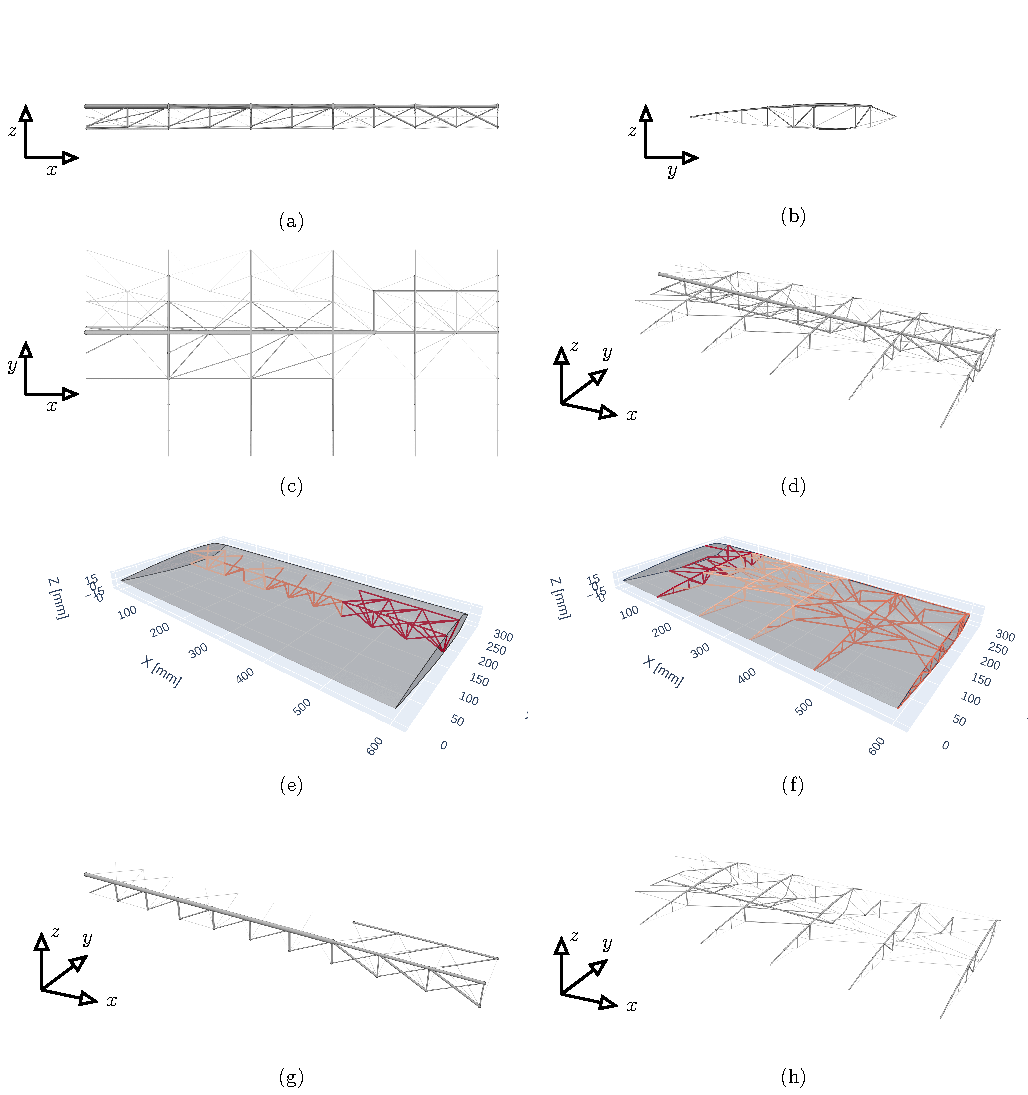
\includegraphics[width=\linewidth]{figures/07_aeronautic/00_NACA_a_sol_3/gs_a.pdf}
        \caption{Subfigures (a) to (d) present different views on the resulting optimized structure obtained for configuration A with $N_\text{T}=3$ different topologies for the wingbox and the section type modules. The structure has a total mass of $M=\qty{29.5}{\gram}$ and a mass density of $\bar{\rho}=\qty{6.93}{kg/m^3}$; (e) and (f) illustrates the modules' layout in the structure for the wingbox and section modules type; (g) and (h) present the modules' topology for the wingbox and section modules type.}
    \label{fig:07_naca_sol_a_nt3}
\end{figure*}

We will now provide a detailed commentary on the topology of the least voluminous solution obtained for $N_\text{T}=3$, with a mass of $M=\qty{29.5}{g}$. \figref{fig:07_naca_sol_a_nt3} visually presents the most noteworthy aspects of the modular structure. Subfigures (a) to (d) depict the structure from four different angles. Starting from the root (left part of the images) and progressing towards the tip, we observe distinct features of the topology. Near the root of the wing, the algorithm minimizes the number of members as all nodes are fixed. Moving towards the central part of the wing, the topology resembles a classic wing configuration consisting of spars and ribs. A large spar runs along the entire span of the wing, in the upper half chord. In the initial sections, this spar is composed of tick bars due to high compression loads on the upper skin of the wing. However, towards the wing tip, the single massive spar is split into two thinner spars as the loads decrease.

Examining the ribs, we note that their thickness remains mostly constant regardless of their position on the X-axis. This is because the ribs primarily transfer loads to the larger spars and do not bear additional loads from subsequent sections, as the spars do. However, for wings with different planforms and lift distributions along the X-axis, this uniformity in rib thickness may not be optimal. Shorter ribs, experiencing lower loads, may require thinner dimensions. 

Regarding the layout of the modules, \figref{fig:07_naca_sol_a_nt3}e and \figref{fig:07_naca_sol_a_nt3}f illustrate how the algorithm suggests similar but not identical layout strategies for the two module types. For the wingbox type (\figref{fig:07_naca_sol_a_nt3}e), there is an almost uniform distribution of different module topologies over the wing span, with one notable exception: the fourth subdomain from the root displays a different topology. This deviation could be attributed to either resolving a connectivity issue with neighboring subdomains or the optimizer converging to a local minimum. In the case of the section type (\figref{fig:07_naca_sol_a_nt3}f), the first subdomains near the root exhibit a distinct topology compared to the others. This variation is understandable as these subdomains typically experience different load states due to their proximity to the boundary conditions. This phenomenon aligns with our previous observations, as seen in \figref{fig:06_diferent_modules_cant_topology}, where subdomains near the loads exhibited different topologies. The remaining module topologies are more evenly distributed across the wing span. Finally, in \figref{fig:07_naca_sol_a_nt3}g and \figref{fig:07_naca_sol_a_nt3}h, we present the topology of the two module types separately, the wingbox type and the section type subdomains.

\begin{figure}
    \centering
    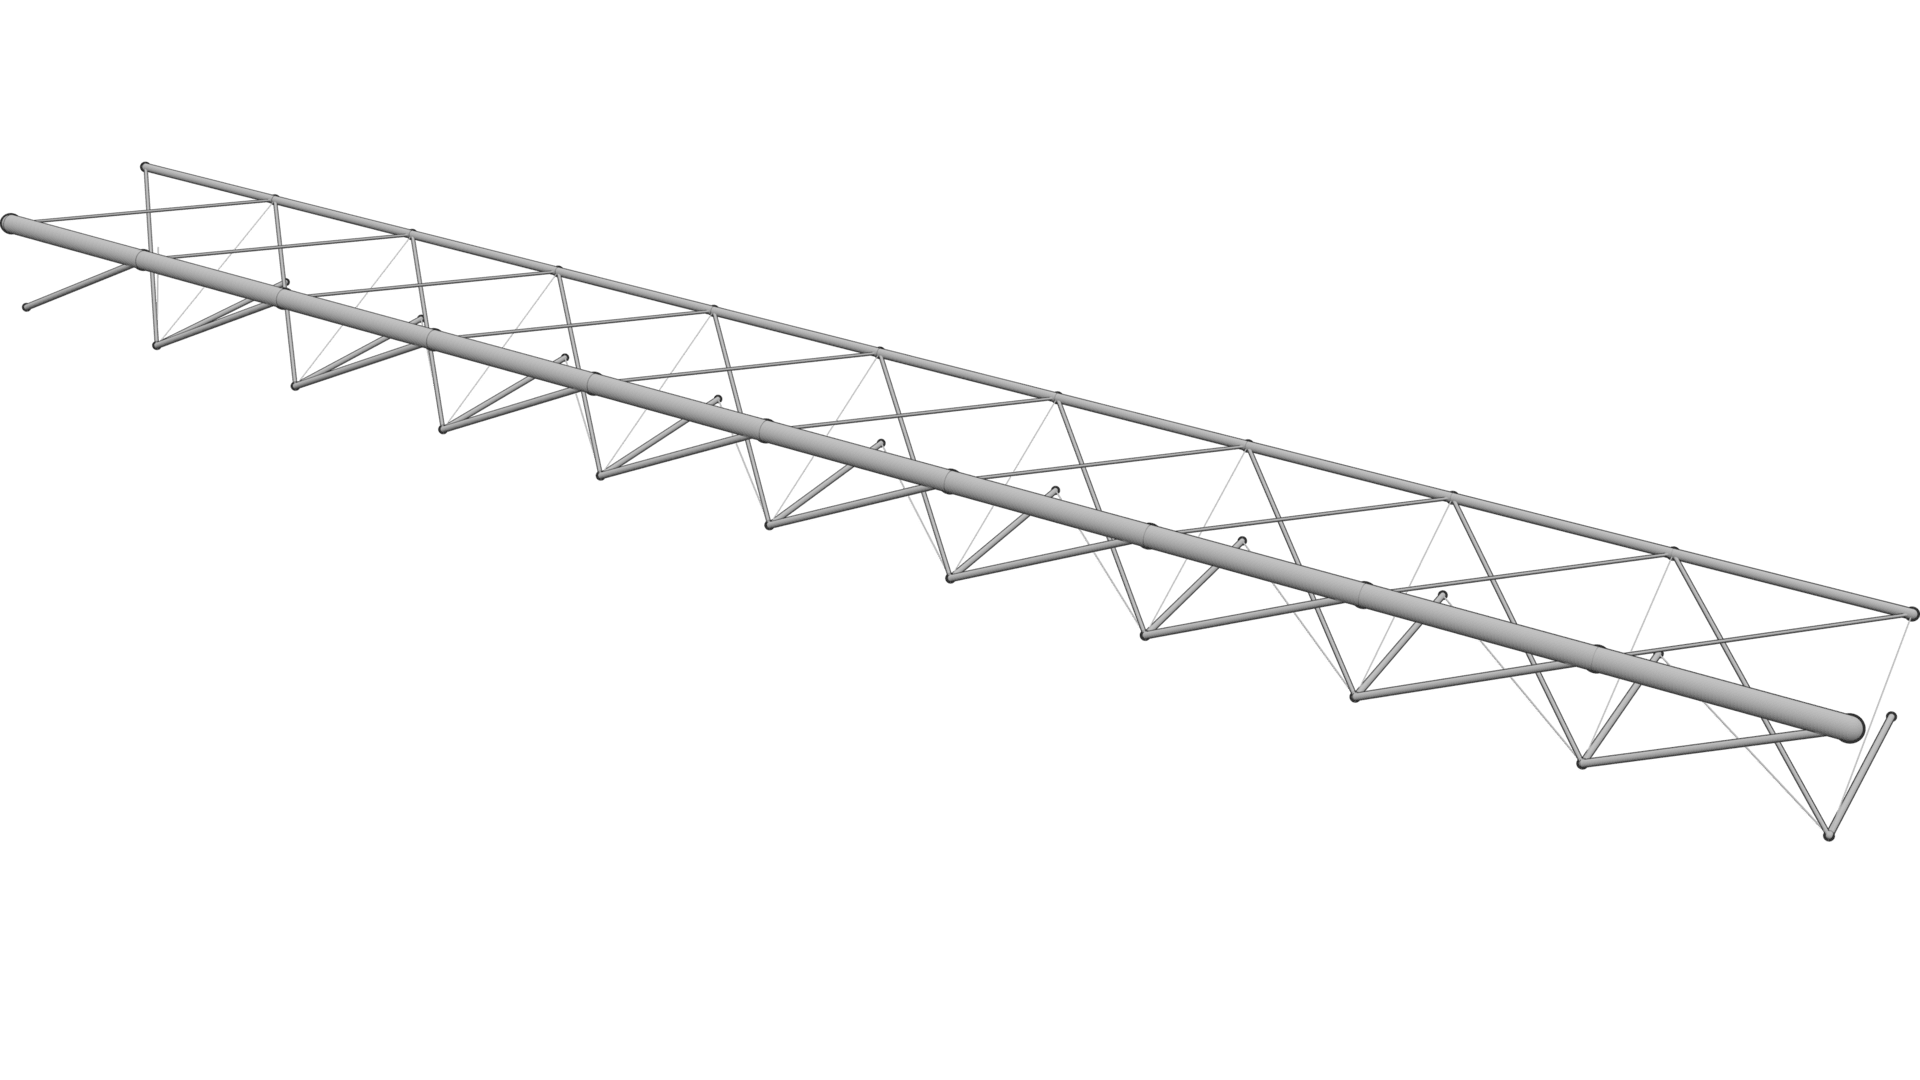
\includegraphics[width=0.8\linewidth]{figures/07_aeronautic/00_NACA_c_1/04_Topology_cell_iso.png}
        \caption{Rendering of the wingbox type subdomains of the resulting optimized structure obtained for configuration A with $N_\text{T}=1$.}
    \label{fig:07_wingbox_a_nt1}
\end{figure}

We have now a closer look at the solution topology of the wingbox type plot in \figref{fig:07_naca_sol_a_nt3}g. It is interesting to note that the structure is characterized by a very voluminous component in the upper part of the wingbox, that resembles a spar. This same component is similarly seen when examining the wingbox type optimized structure for the case with $N_\text{T}=1$ shown in \figref{fig:07_wingbox_a_nt1}. Considering that the cross-sectional area of the spar loaded in compression is particularly sensitive to the free buckling length of the members composing it, we wonder if modifying the ground structure could be beneficial for this specific load case.

For that reason, we decided to test a different ground structure configuration, doubling the number of modules for the wingbox type, effectively halving the maximum length of the bars under compressive loading. The new wingbox ground structure is shown in \figref{fig:07_gs_wingbox_b}. A comparison with \figref{fig:07_gs_a_types}b shows that the ground structure becomes naturally denser.  The section type ground structure becomes denser as well even though the generation parameters were unchanged. This fact is due to the two ground structures being conformal. We refer to this modified ground structure configuration as configuration B.

\begin{figure}
    \centering
    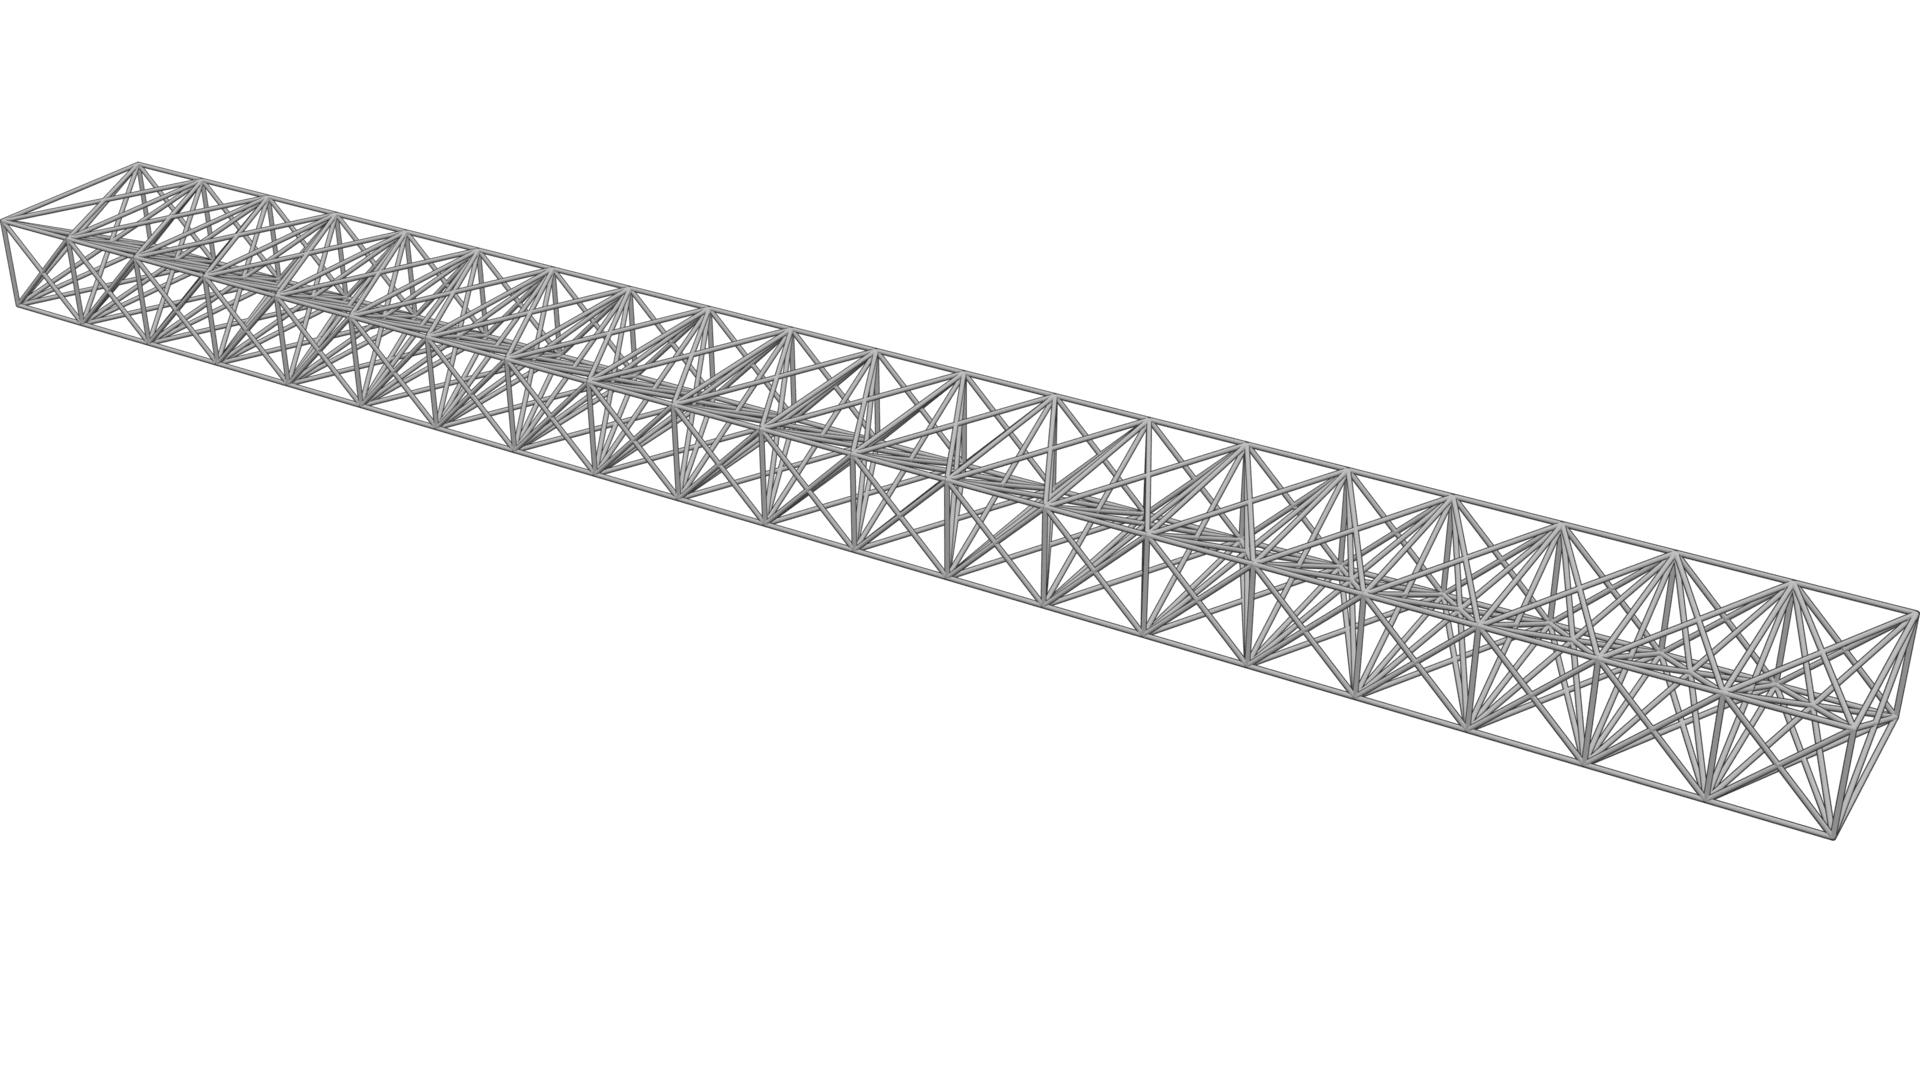
\includegraphics[width=0.8\linewidth]{figures/07_aeronautic/00_NACA_gs_b/02_GS_c_iso.png}
        \caption{Visual representation of the ground structure of the 20 wingbox type subdomains of configuration B.}
    \label{fig:07_gs_wingbox_b}
\end{figure}

The numerical results of the optimizations for configuration B are presented in the right-hand side part of \tabref{tab:07_naca_num_res}. As correctly predicted, reducing the free effective buckling length of the members that compose the main wing spar considerably helped to reduce the mass of the structure. We observe a \qty{23}{\percent}, \qty{28}{\percent}, and \qty{22}{\percent} reduction in mass compared to configuration A, for the three values of $N_\text{T}$ respectively. The volume trends for the two configurations are plotted in \figref{fig:07_mass_b}. It is important to remember that in \secref{sec:05_doe}, we observed that increasing the number of subdomains tends to increase the volume of the solution, but in this specific test case, we observe a different behavior. This fact confirms that choosing the correct ground structure is critical to obtaining a good solution. Finally, despite the increase in candidate members, the optimization times of configuration B cases remained the same, with no optimization exceeding five minutes of calculation time.

\begin{marginfigure}
    \centering
    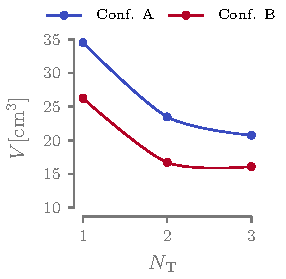
\includegraphics[width=\linewidth]{figures/07_aeronautic/00_NACA_vol_crv/vol.pdf}
    \caption{Evolution of the mass of the NACA 0012 \gls{uav} wing structure for configuration A and B and different number of modules' topologies $N_\text{T}$.}
    \label{fig:07_mass_b}
\end{marginfigure}

Finally, in \figref{fig:07_topology_naca_b}, we present the resulting optimized structure obtained for configuration B with $N_\text{T}=3$ for both the wingbox and the section type modules. The structure has a total mass of $M=\qty{22.9}{\gram}$ and a mass density of $\bar{\rho}=\qty{5.38}{kg/m^3}$. \figref{fig:07_topology_naca_b}a shows the isometric view of the optimized topology. The structure exhibits similar characteristics to the configuration case A, with uniform ribs and a single large spar that splits into two towards the end of the span. However, the difference becomes apparent when observing the wingbox type subdomains in \figref{fig:07_topology_naca_b}b and \figref{fig:07_topology_naca_b}d. Here, we observe how the reduced buckling length of the bars, given by the higher number of subdomains, helps in reducing the cross-sectional area of the large spar. The layout of the modules is depicted in \figref{fig:07_topology_naca_b}b and \figref{fig:07_topology_naca_b}c for the two module types. Compared to the results of configuration A, we notice a more even distribution.

\begin{figure*}
    \centering
    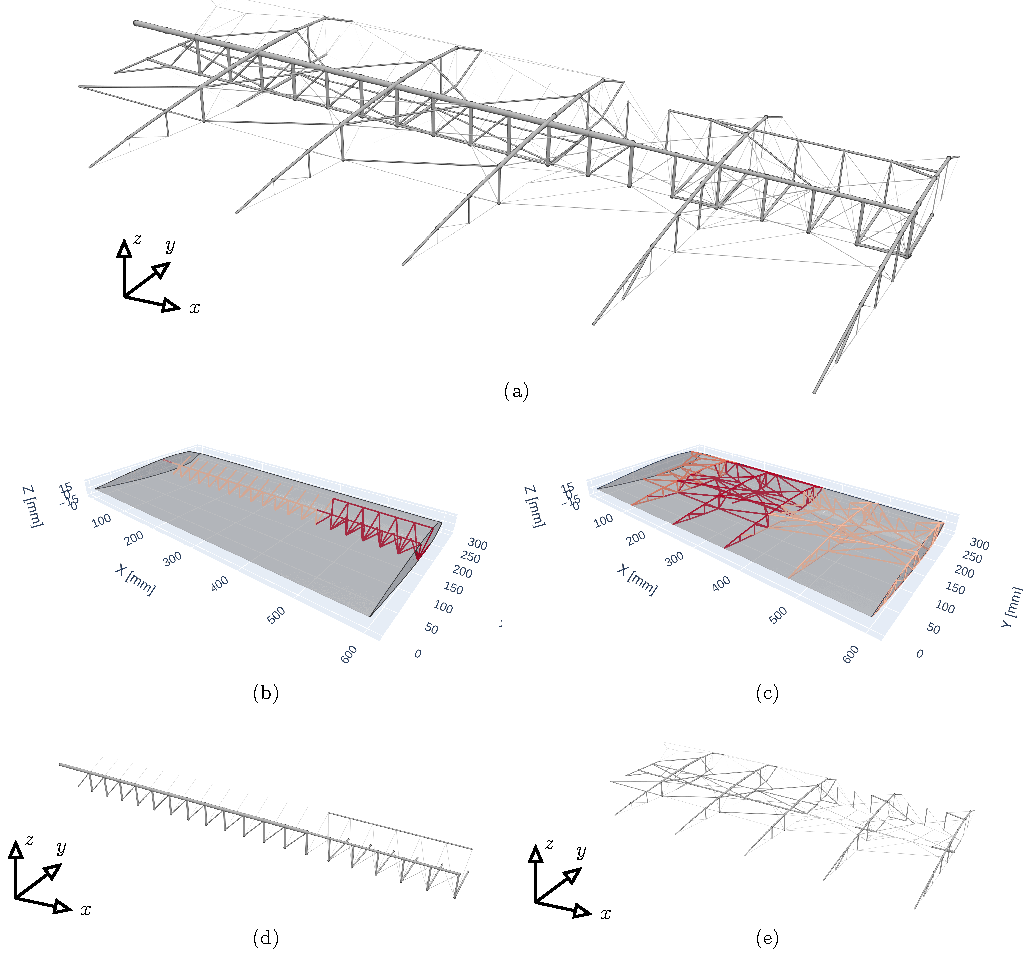
\includegraphics[width=\linewidth]{figures/07_aeronautic/00_NACA_b_sol_3/gs_a.pdf}
        \caption{Subfigures (a) presents the resulting optimized structure obtained for configuration B with $N_\text{T}=3$ different topologies for the wingbox and the section type modules. The structure has a total mass of $M=\qty{22.9}{\gram}$ and a mass density of $\bar{\rho}=\qty{5.38}{kg/m^3}$; (b) and (c) illustrates the modules' layout in the structure for the wingbox and section modules type; (d) and (e) present the modules' topology for the wingbox and section modules type.}
    \label{fig:07_topology_naca_b}
\end{figure*}

\section{Conclusion}
In this chapter, we focused on studying the applicability of the optimization algorithms proposed in this thesis in real engineering test cases, with real dimensions, loads, and materials. Firstly, we benchmarked the monolithic optimization algorithm proposed in \chpref{chap:04} using a three-load-case test case on the CRM structure. We achieved a \qty{27}{\percent} lighter structure compared to the literature, employing a gradient-based optimizer that solved the problem in minutes instead of days. Additionally, we performed further tests on the structure, evaluating the influence of displacement constraints, material data, and the fineness of the initial ground structure.

Secondly, we performed the optimization of a modular \gls{uav} wing structure based on the NACA 0012 profile. We developed an algorithm that allows the generation of modular ground structures starting from any volume. Then, we used this algorithm to generate the ground structure of the NACA 0012 volume, subdividing the structure into two module types. We studied how the optimized structure changed with the variation of the number of topologies. Additionally, we proposed a better ground structure configuration based on engineering observations and confirmed that the starting ground structure can influence the solution.